\documentclass{article}
\usepackage{graphicx}
\usepackage[a4paper, margin=0.8in]{geometry}
\usepackage{subcaption}
\usepackage{caption}
\usepackage{float}
\usepackage{hyperref}
\hypersetup{
    colorlinks=true,      % false: boxed links; true: colored links
    linkcolor=blue,       % color of internal links
    citecolor=blue,       % color of links to bibliography
    filecolor=blue,       % color of file links
    urlcolor=blue         % color of external links
}

\title{COL334 Assignment 1}
\author{Yash Bansal \\ 2022CS51133}

\begin{document}

\maketitle

\section{Measurement tools}

\subsection{Ping}

\subsubsection{Part A}
\begin{figure}[H]
    \centering
    \begin{subfigure}[b]{0.48\textwidth}
        \centering
        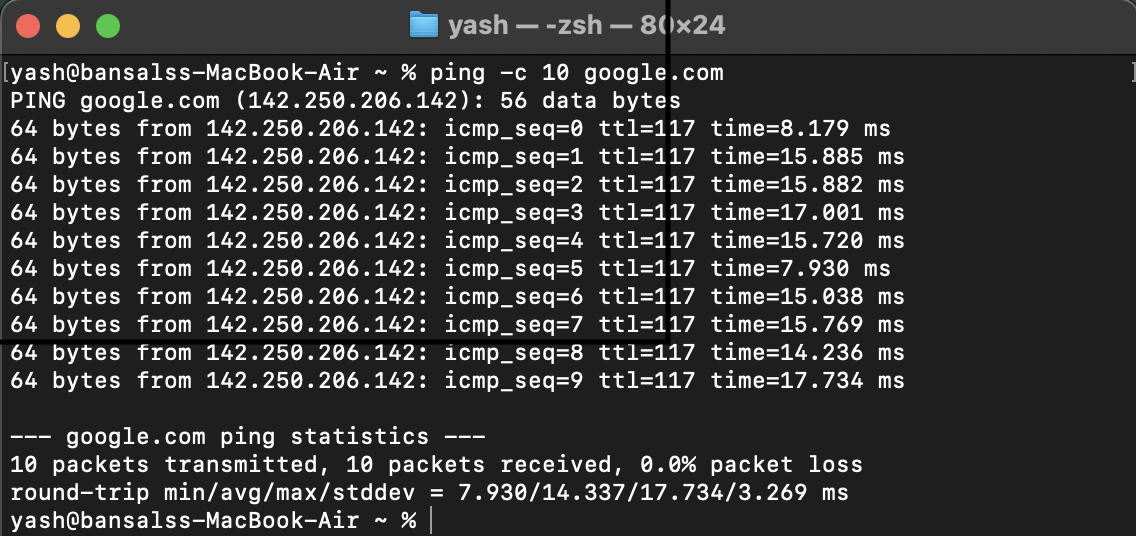
\includegraphics[width=\textwidth]{ping_google_iitd_ipv4.png}
        \caption*{\textbf{google.com:} avg. ping:- 14.33 ms}
    \end{subfigure}
    \hfill
    \begin{subfigure}[b]{0.48\textwidth}
        \centering
        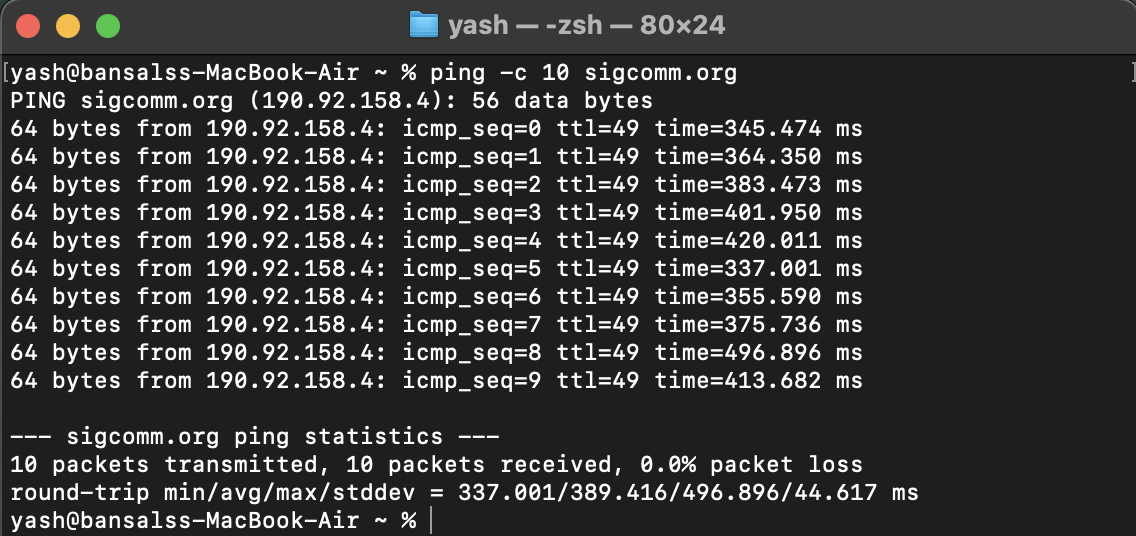
\includegraphics[width=\textwidth]{ping_sigcomm_iitd_ipv4.png}
        \caption*{\textbf{sigcomm.org:} avg. ping:- 389.41 ms}
    \end{subfigure}
    \caption*{Ping from IITD Network using IPv4}
\end{figure}

\begin{figure}[H]
    \centering
    \begin{subfigure}[b]{0.48\textwidth}
        \centering
        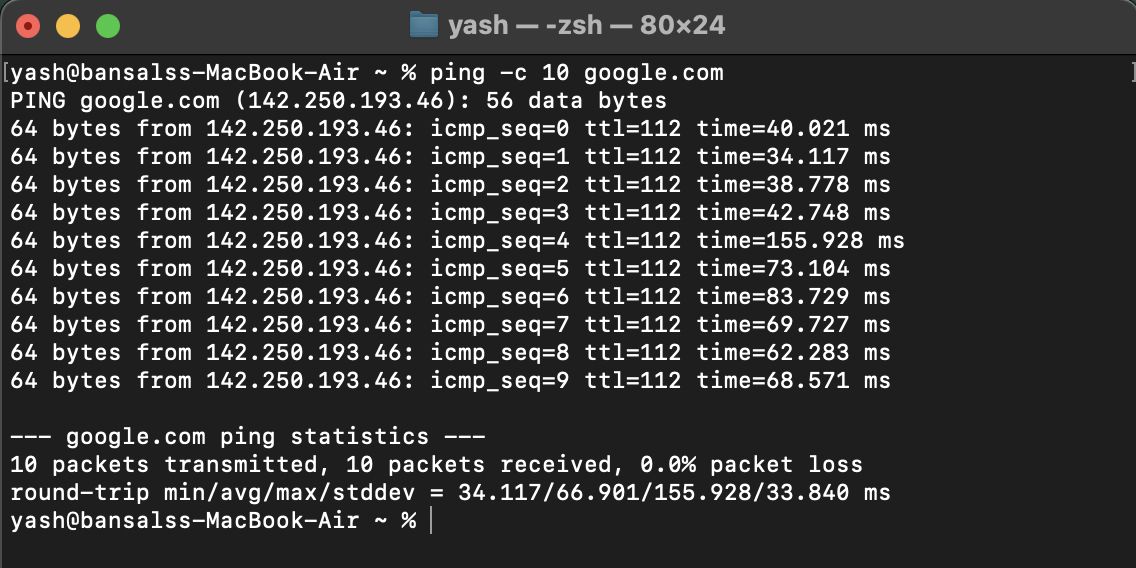
\includegraphics[width=\textwidth]{ping_google_personal_ipv4.png}
        \caption*{\textbf{google.com:} avg. ping:- 66.90 ms}
    \end{subfigure}
    \hfill
    \begin{subfigure}[b]{0.48\textwidth}
        \centering
        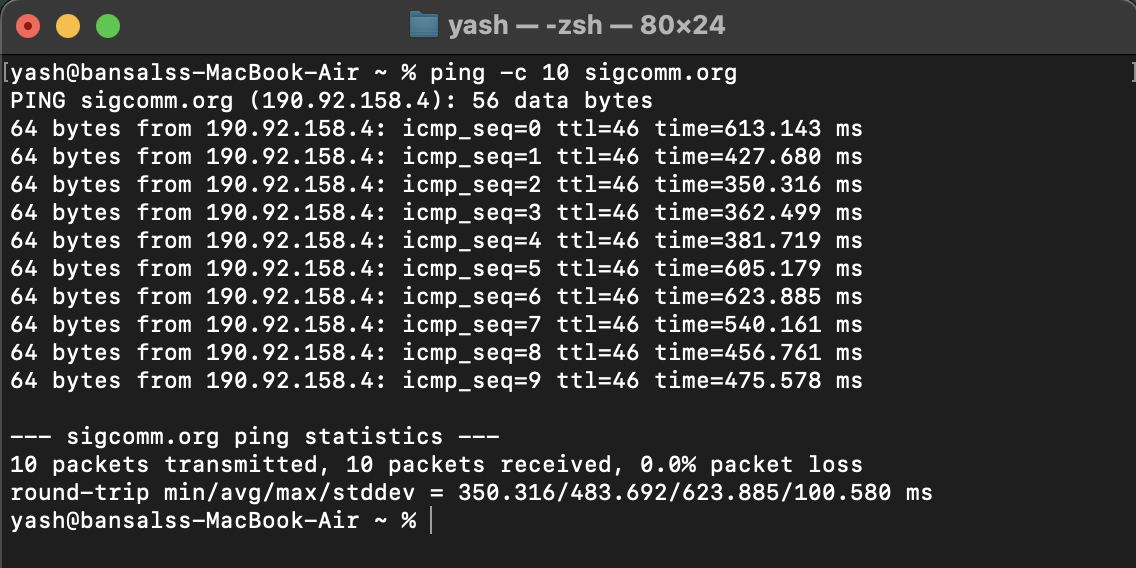
\includegraphics[width=\textwidth]{ping_sigcomm_personal_ipv4.png}
        \caption*{\textbf{sigcomm.org:} avg. ping:- 483.69 ms}
    \end{subfigure}
    \caption*{Ping from personal network using IPv4}
\end{figure}

\textbf{Observations}:-
\begin{enumerate}
    \item The average ping latency for sigcomm.org is much higher than that of google.com. It could be because, on referring to traceroute results, fewer hops are required to reach google.com for both networks, as compared to sigcomm.org.
        \begin{itemize}
        \item One reason for this can be peering with many networks by Google, which results in a smaller route. 
        \item Also, for sigcomm.org, there are a set of last few hopes having similar IP addresses, which have a huge latency for traceroute. So, this slower internal network of sigcomm.org results in a higher ping.
        \end{itemize}
    \item The average ping latency for the IITD network is less than that of the personal network for both websites. 
        \begin{itemize}
            \item It is because, on seeing traceroute results, the IITD network is taking fewer hops to reach the destination website than the personal network, resulting in low ping latency for the IITD network.
            \item Another reason could be the bandwidth of the network. IITD networks have higher individual bandwidth than personal networks, which have lower individual bandwidth due to more users.
        \end{itemize}
\end{enumerate}

\subsubsection{Part B}
\begin{enumerate}
    \item The ping commands in the attached screenshots above use item IPv4 and ICMP(Internet Control Message Protocol) protocols. The following attached wireshark screenshot for the ping packet can also verify it.
    
        \begin{figure}[ht]
        \centering
        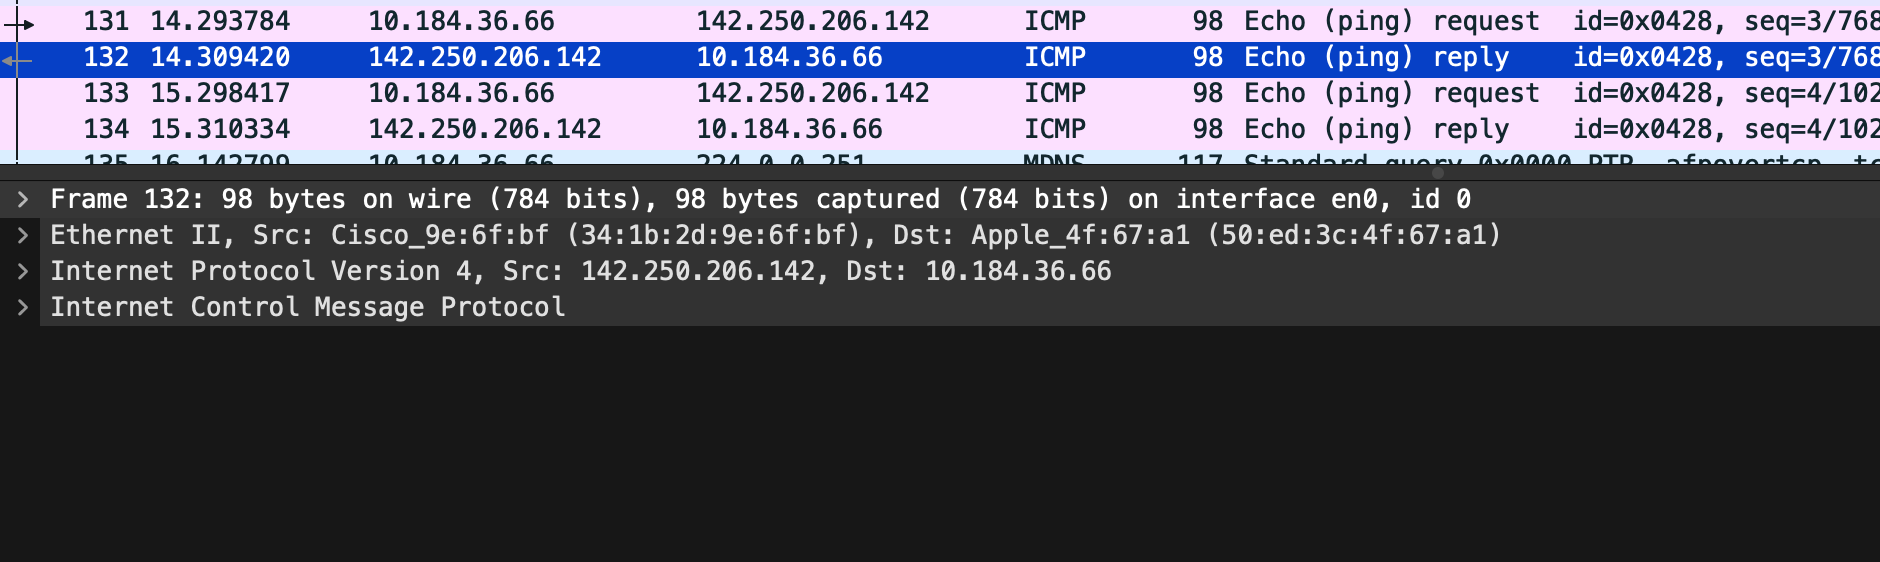
\includegraphics[width=0.9\textwidth]{ping_wireshark.png}
        \caption*{Wireshark screenshot for google.com ping packet}
        \end{figure}
    
        \begin{itemize}
            \item When using ping, an ICMP echo request packet is sent to the target IP address. It requests the target to send an ICMP echo reply.
            \item After the reply packet is received, the source machine calculates the round-trip time(RTT) to return the ping latency.
            \item If the destination source is unavailable/configured not to reply to ICMP echo request, the request timed out is shown by the source machine.
            \item All these addressing and routings are done using the IPv4 protocol, so changing the network protocol can also change the ping latency due to efficient headers and implementations.
        \end{itemize}

    \item The packet size for the ping requests is 64 bytes using IPv4 ping protocol (98 bytes, including headers, as detected by Wireshark). 
    \begin{itemize}
        \item The maximum packet size for an IPv4 packet can be 65,535 bytes with a 28-byte header. So, theoretically, ping packets can be as large as 65,507 bytes. But, normally, we need to keep the packet size as small as possible, as we need the RTT using ping, so just the required data is kept in the ping packet, namely source and destination IPs and the protocol headers.
        \item No, I cannot ping with theoretical maximum packet size, as it is just theoretically achievable. Various other factors must be considered, like hardware limits in routers and switches, errors using larger packets, header size, etc.
        
    \end{itemize}
\end{enumerate}

\subsubsection{Part C}
Ping using IPv6 can be done by just changing the command from ping to ping6 in the terminal. The following wireshark screenshot can verify the protocols used.
        \begin{figure}[ht]
        \centering
        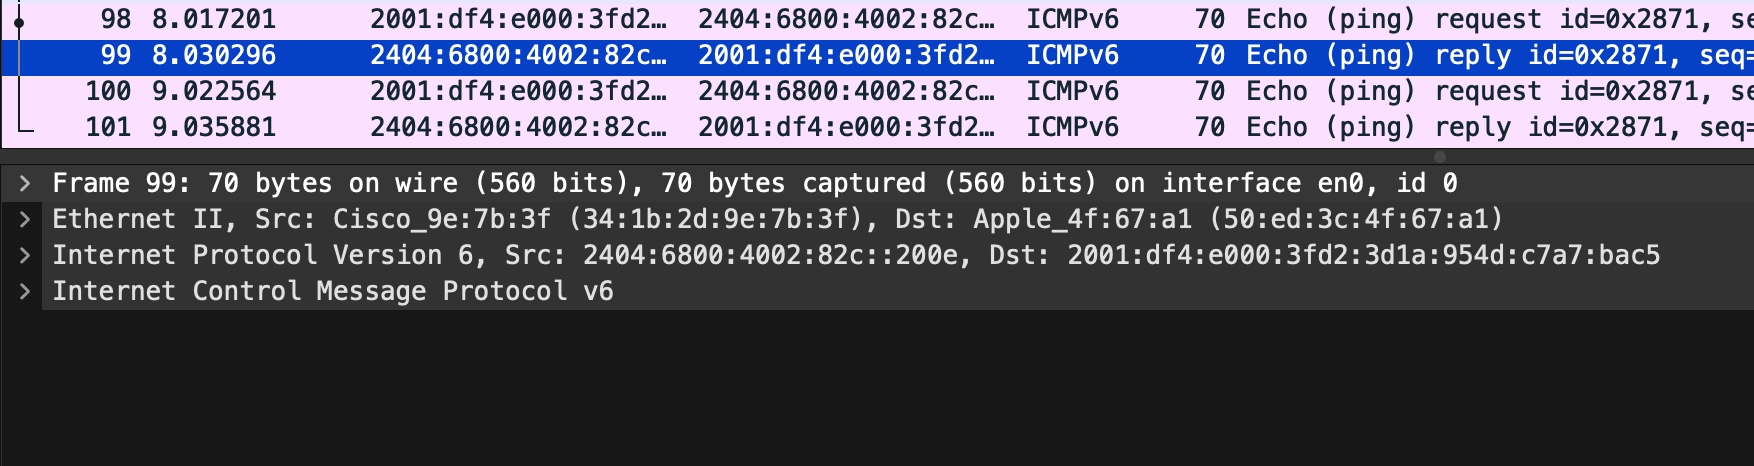
\includegraphics[width=0.9\textwidth]{ping6_wireshark.png}
        \caption*{Wireshark screenshot for google.com ping packet using IPv6}
        \end{figure}

\begin{figure}[H]
    \centering
    \begin{subfigure}[b]{0.48\textwidth}
        \centering
        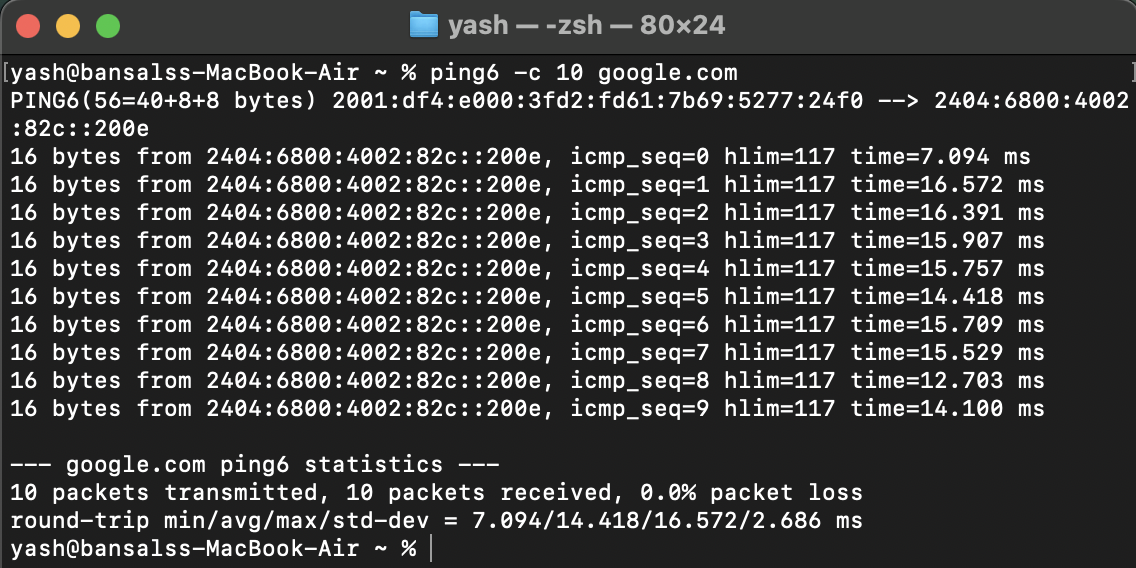
\includegraphics[width=\textwidth]{ping_google_iitd_ipv6.png}
        \caption*{\textbf{google.com:} avg. ping:- 14.41 ms}
    \end{subfigure}
    \hfill
    \begin{subfigure}[b]{0.48\textwidth}
        \centering
        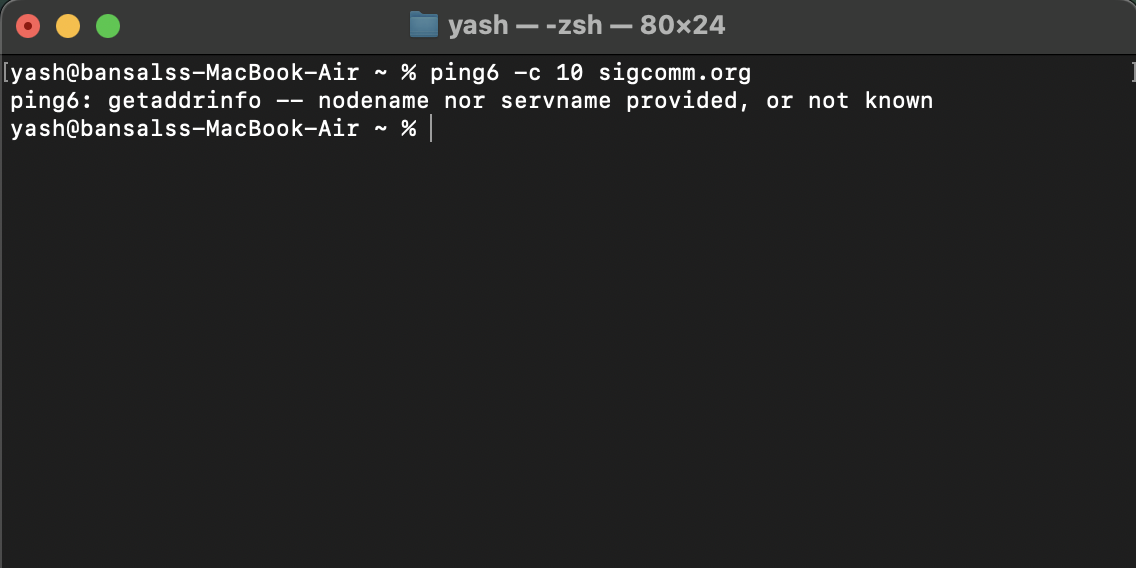
\includegraphics[width=\textwidth]{ping_sigcomm_iitd_ipv6.png}
        \caption*{\textbf{sigcomm.org:} Unable to ping}
    \end{subfigure}
    \caption*{Ping from IITD Network using IPv6}
\end{figure}

\begin{figure}[H]
    \centering
    \begin{subfigure}[b]{0.48\textwidth}
        \centering
        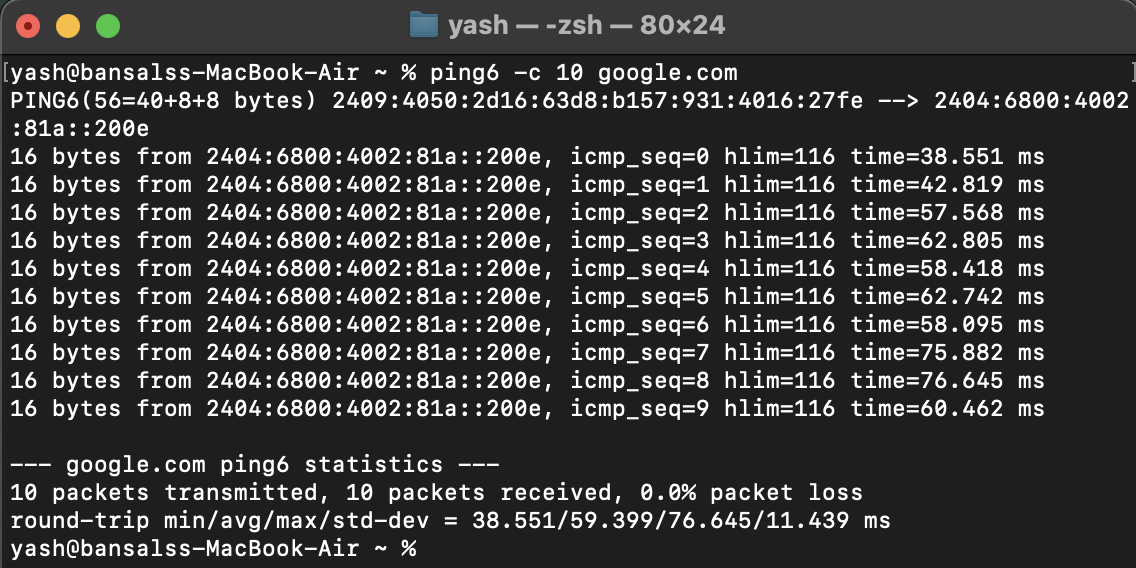
\includegraphics[width=\textwidth]{ping_google_personal_ipv6.png}
        \caption*{\textbf{google.com:} avg. ping:- 59.39 ms}
    \end{subfigure}
    \hfill
    \begin{subfigure}[b]{0.48\textwidth}
        \centering
        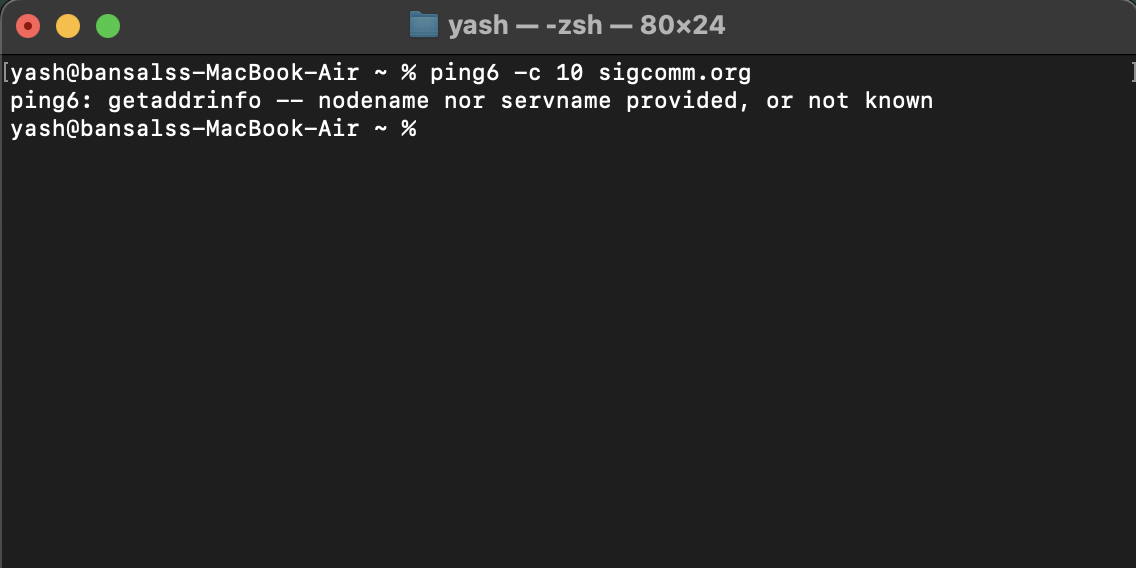
\includegraphics[width=\textwidth]{ping_sigcomm_personal_ipv6.png}
        \caption*{\textbf{sigcomm.org:} Unable to ping}
    \end{subfigure}
    \caption*{Ping from personal network using IPv6}
\end{figure}

\textbf{Observations:- }
\begin{enumerate}
    \item For google.com, the average ping latency remains almost the same in the case of IPv6. This is because the total number of hops remained the same as for IPv4, both in the case of the IITD Network and personal network, which indicates that the path must have remained the same, just the protocol gets changed.
    \item sigcomm.org cannot be pinged using IPv6, nor can it be routed using IPv6 traceroute. This could be because sigcomm.org still does not support IPv6 in their servers, or there may be no path to sigcomm.org in which all the routers/switches support IPv6 protocol.
    \item The packet size for ping using IPv6 is 16 bytes, which is lower than that of the IPv4 protocol. Also, ICMPv6 is used in IPv6, as compared to ICMP in IPv4.
\end{enumerate}
\newpage
\subsection{Traceroute}
\textbf{A.} The attached screenshots contain the traceroute outputs. Autonomous systems are checked using the whois terminal command.
    \begin{figure}[H]
    \centering
    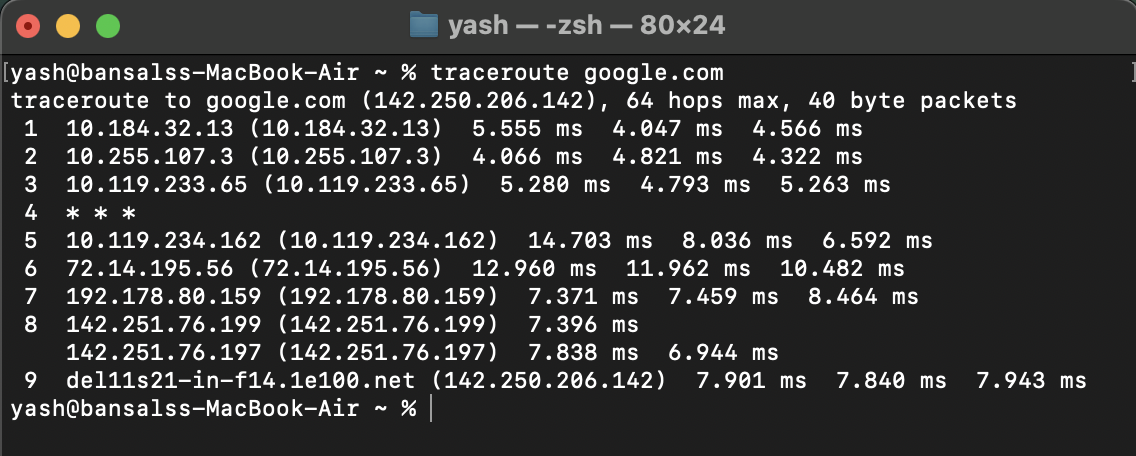
\includegraphics[width=\textwidth]{trace_google_iitd_ipv4.png}
    \caption*{Traceroute to google.com using IITD Network \\
    9 hops, 2 autonomous systems}
    \end{figure}

    \begin{figure}[H]
    \centering
    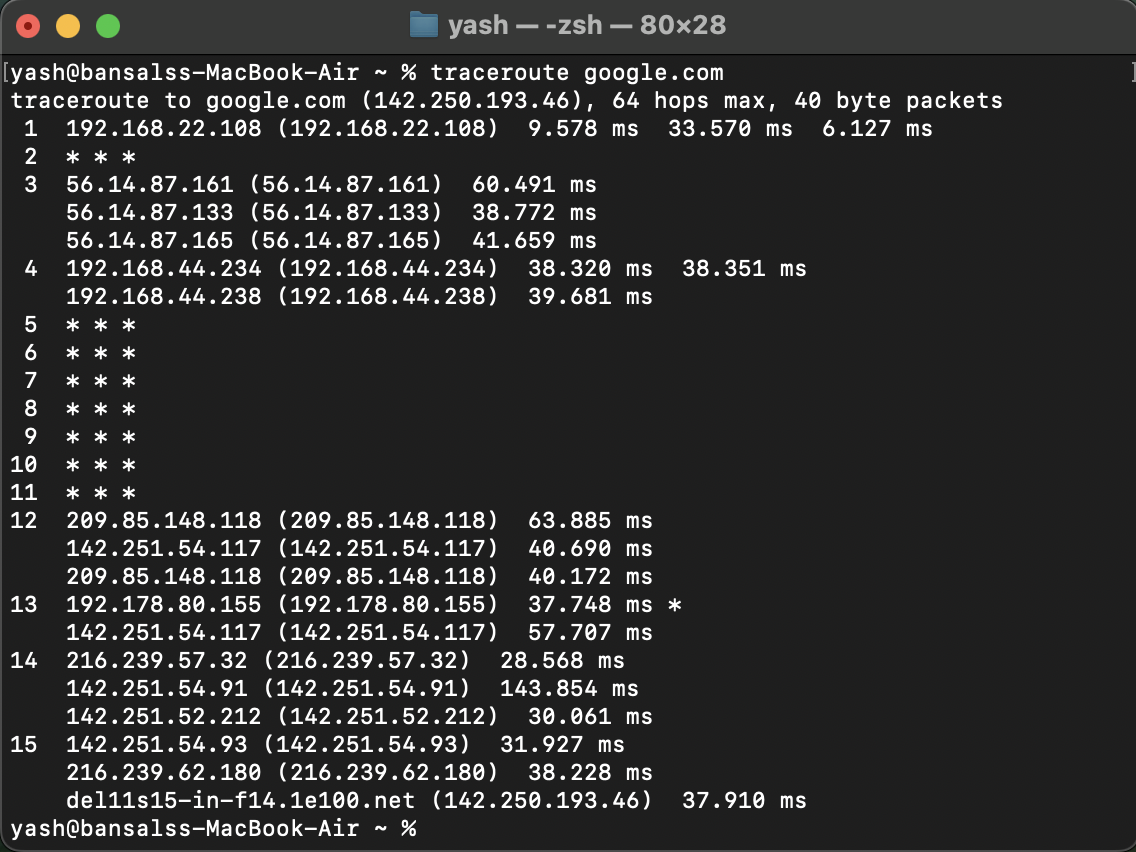
\includegraphics[width=\textwidth]{trace_google_personal_ipv4.png}
    \caption*{Traceroute to google.com using personal network\\
    15 hops, 3 autonomous systems}
    \end{figure}
    
    \begin{figure}[H]
    \centering
    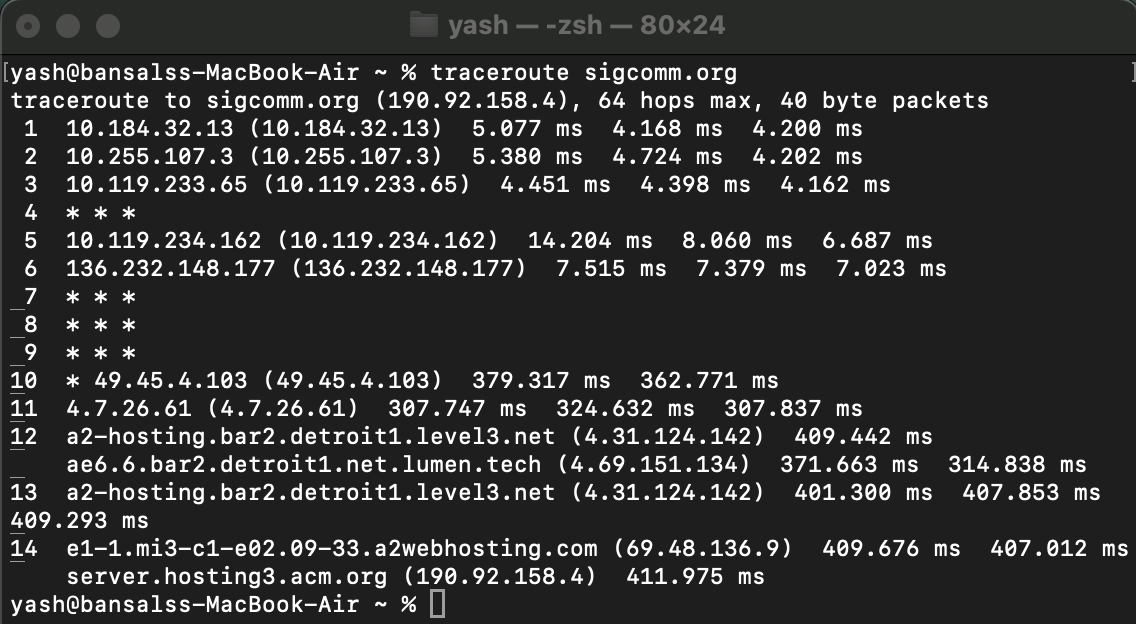
\includegraphics[width=\textwidth]{trace_sigcomm_iitd_ipv4.png}
    \caption*{Traceroute to sigcomm.org using IITD Network\\
    14 hops, 3 autonomous systems}
    \end{figure}

    \begin{figure}[H]
    \centering
    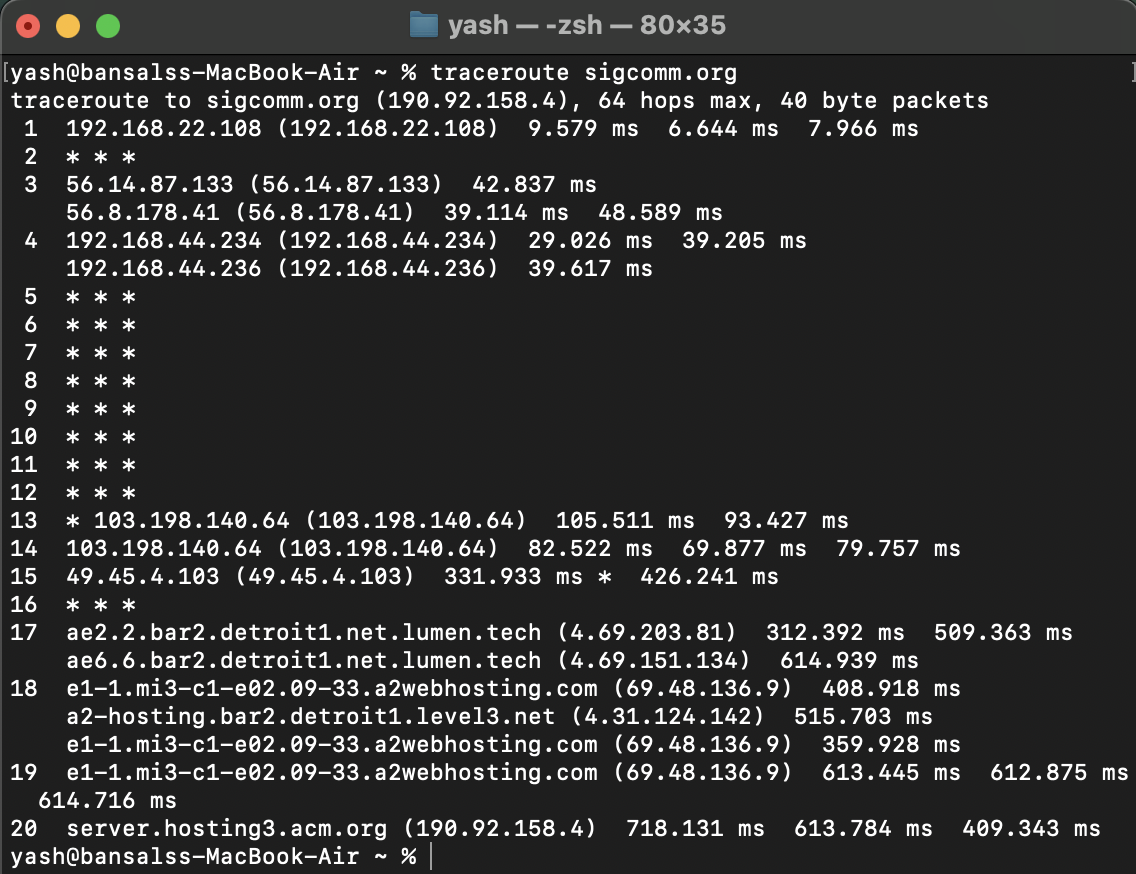
\includegraphics[width=\textwidth]{trace_sigcomm_personal_ipv4.png}
    \caption*{Traceroute to sigcomm.org using personal network\\
    15 hops, 4 autonomous systems}
    \end{figure}

\begin{itemize}
    \item The * output in some IP addresses may be because the system does not receive the required packets from that particular IP address. It could be due to some security policies/blocking of particular ICMP/UDP packets by the systems.
    \item Yes, multiple IP addresses are available for some hop counts. It may be because of multiple servers for load balancing at the particular router or router changes between the packet transfer for faster transmission. It can be noted that the multiple IP addresses of the same hop count belong to the same autonomous system.
    \item The first IP address of the router while tracing google.com using IITD Network is 10.184.32.13. It is the IP address of the router nearest to me. No response can be received by pinging this using a personal network. It could be because IITD has an internal network that any outer service provider cannot access without a VPN.
    \item Yes, I observed a two-tiered structure while tracerouting google.com with IITD Network. It implies that IITD has directly peered with Google. Thus, only two autonomous systems(IITD and Google) are detected in the traceroute. However, while tracerouting with the personal network, a 3-tiered structure was observed. 
    \item For sigcomm.org, multiple autonomous systems are observed in between, which means that the organization has not peered with many organizations. Thus, a longer route with more autonomous systems is detected.

    \textbf{Geolocations:- }

    \begin{figure}[H]
    \centering
    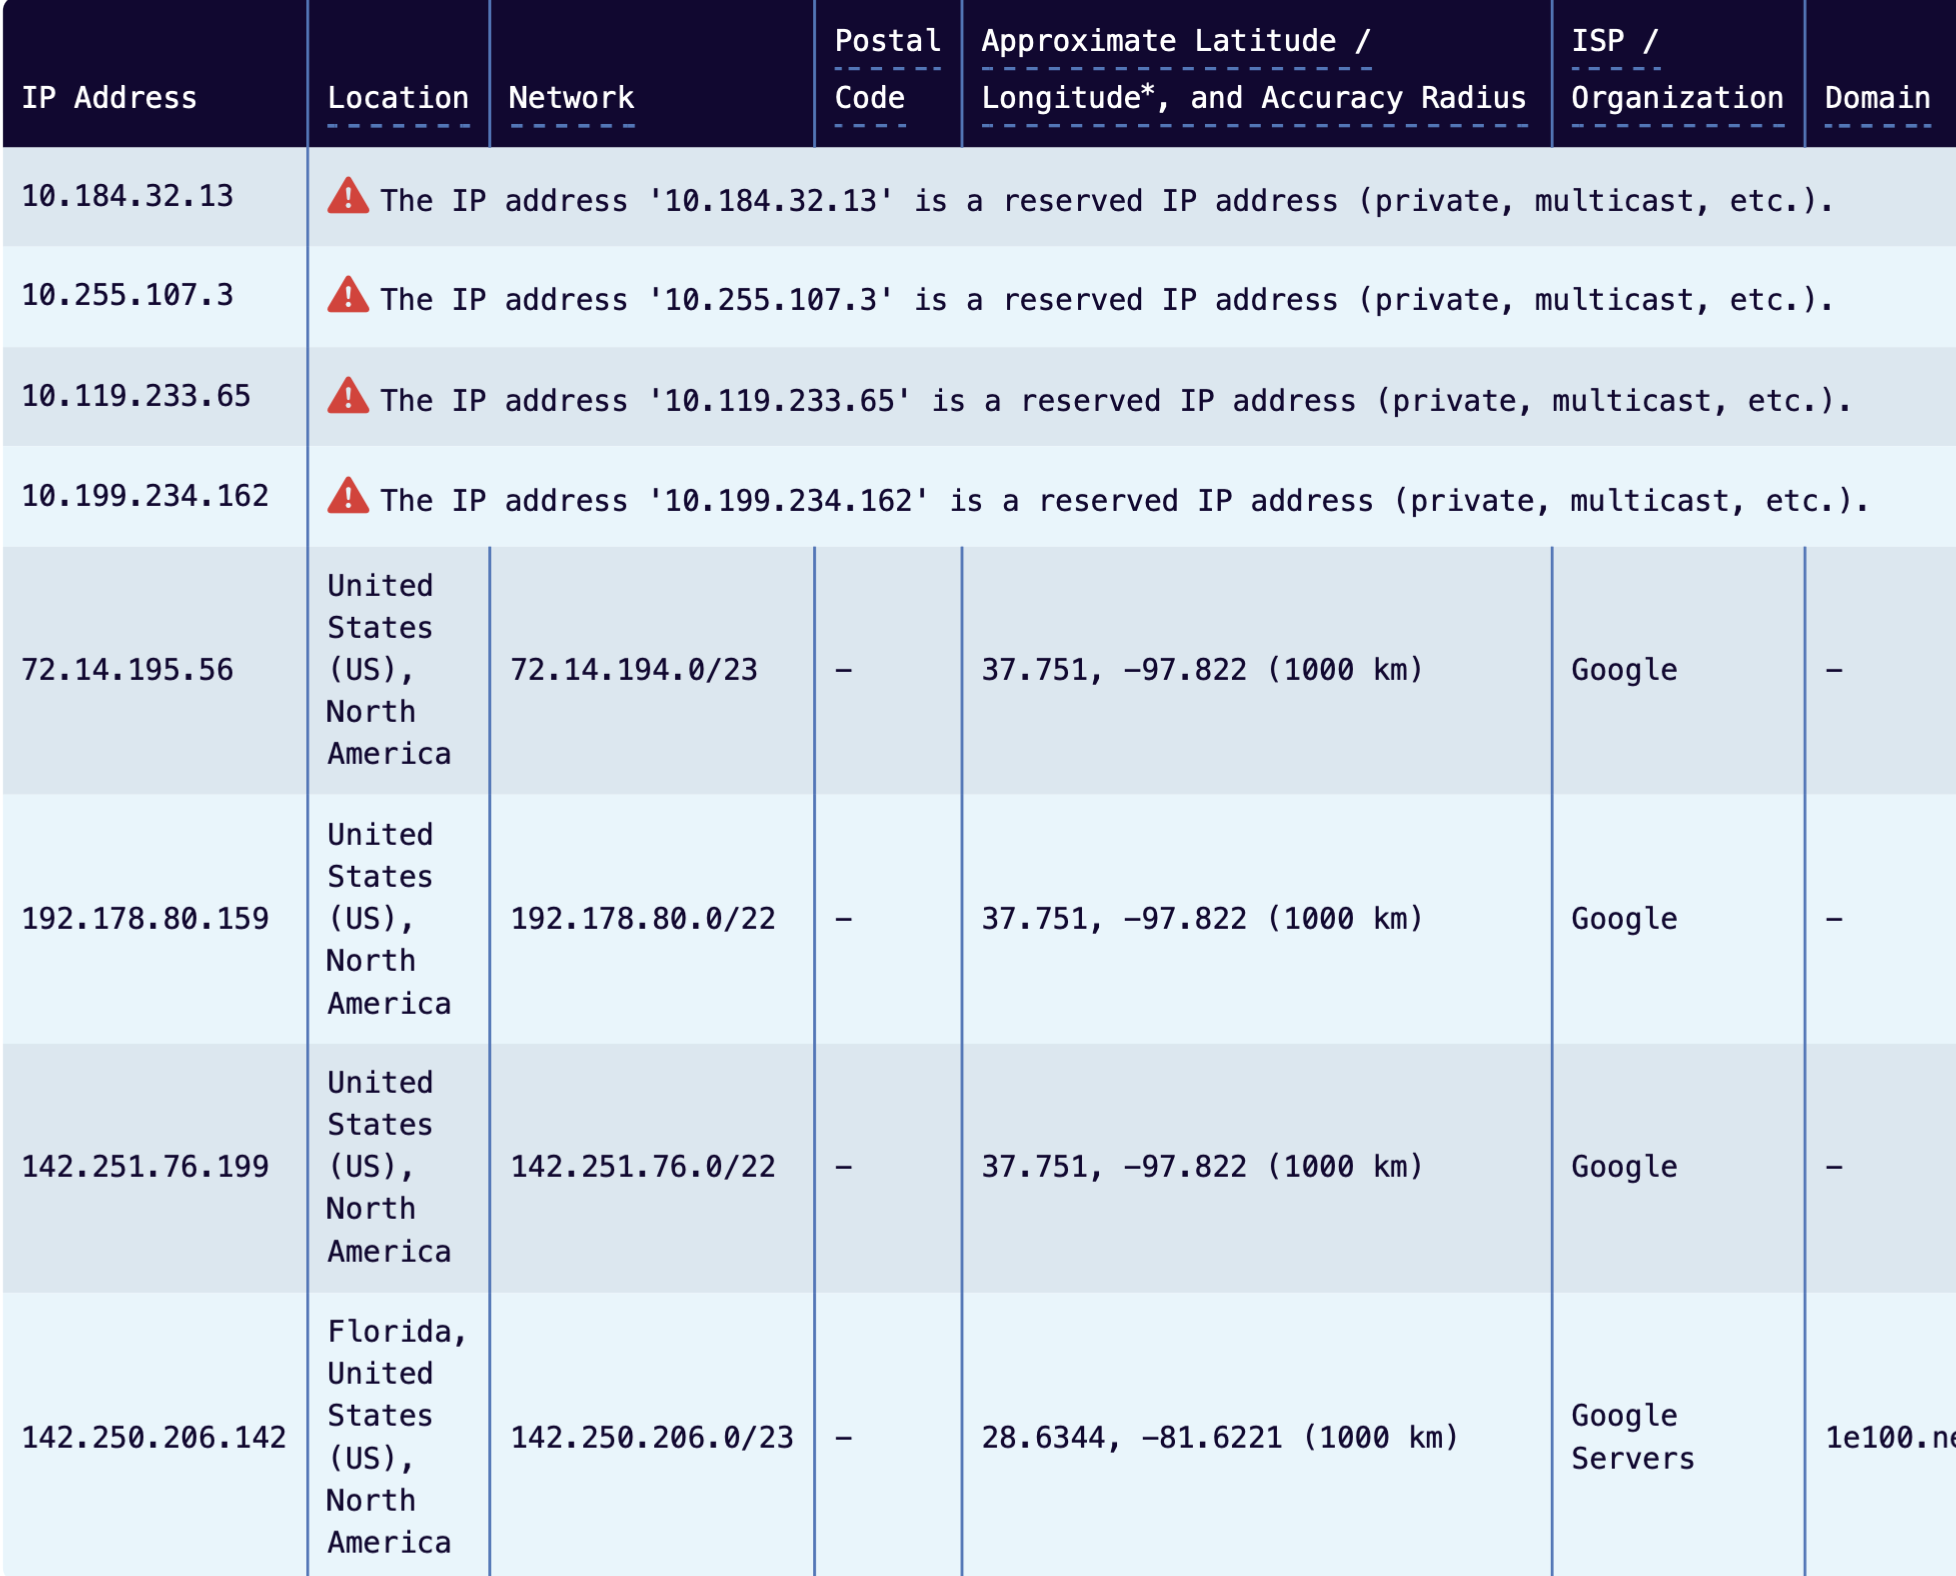
\includegraphics[width=0.9\textwidth]{geolocation_google_IITD.png}
    \caption*{Googlw with IITD Network}
    \end{figure}

    \begin{figure}[H]
    \centering
    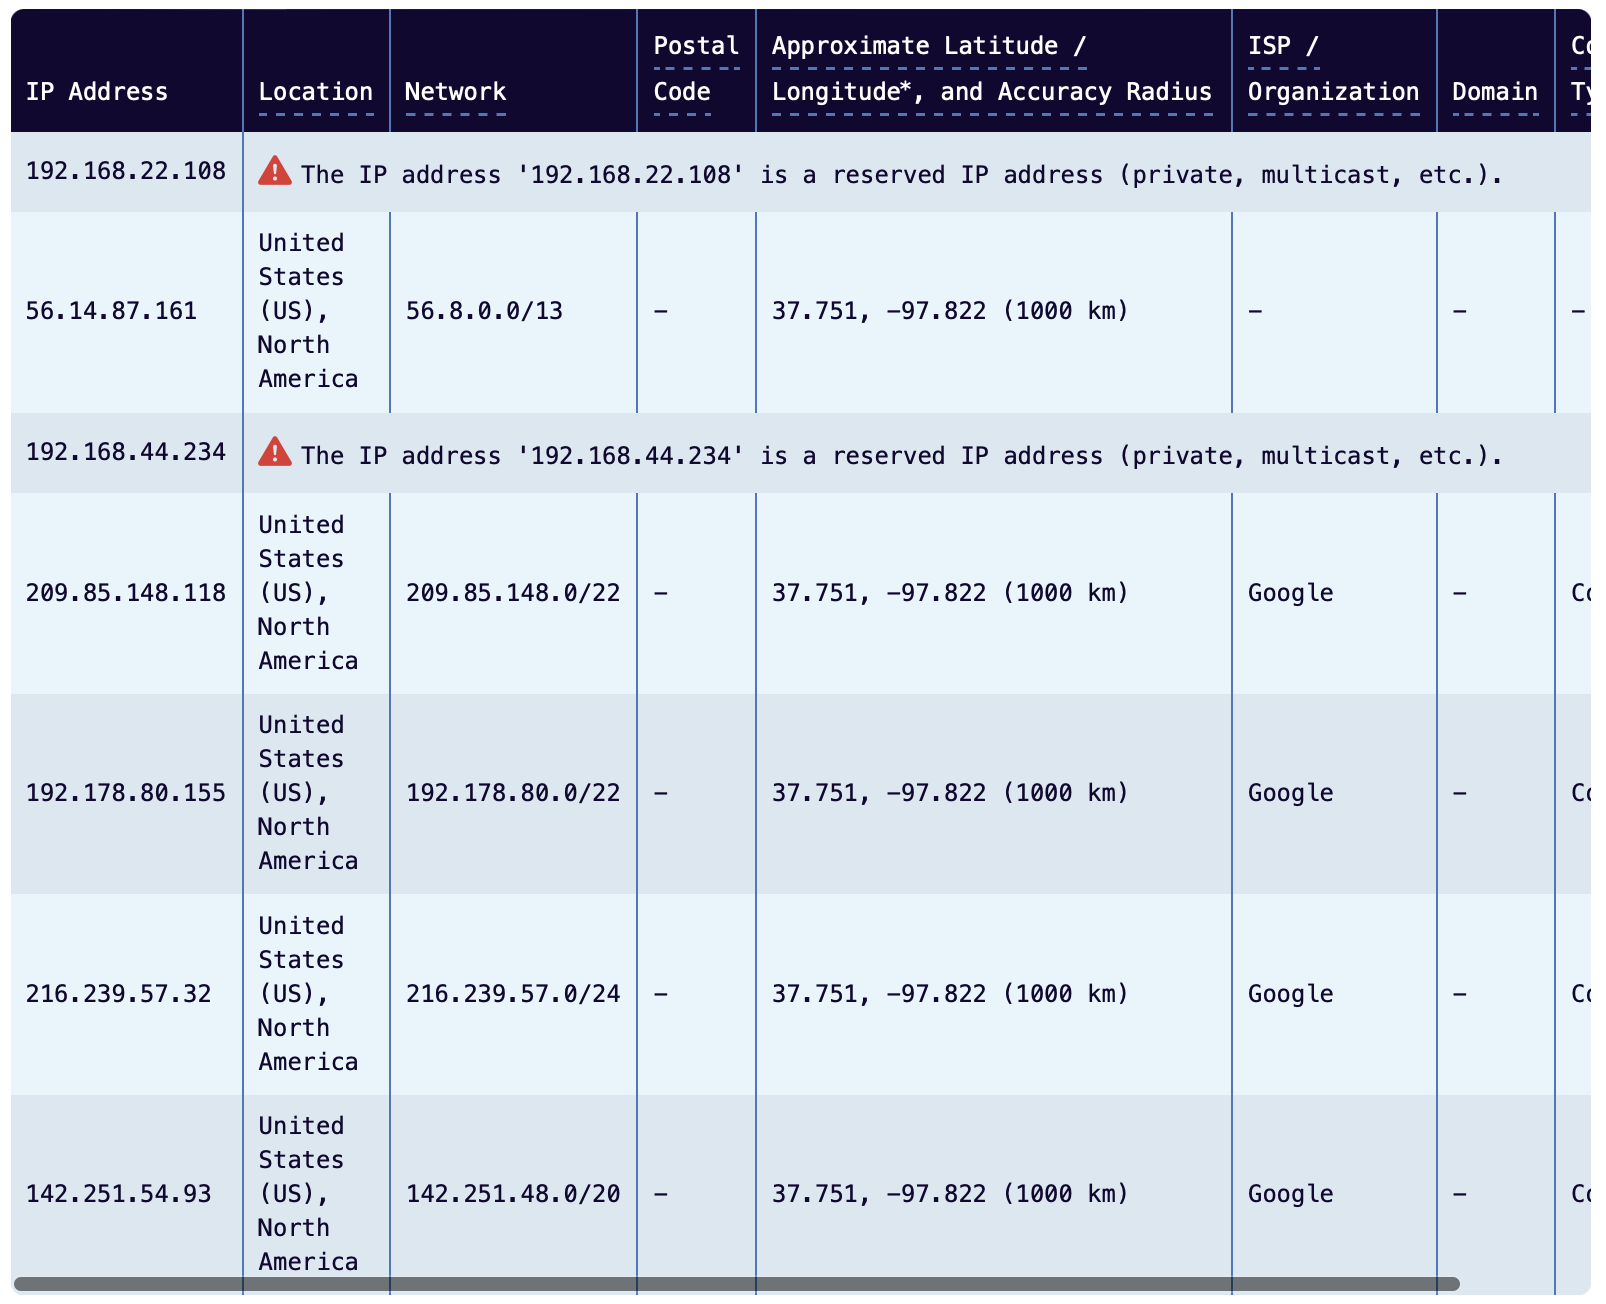
\includegraphics[width=0.9\textwidth]{geolocation_google_personal.png}
    \caption*{Google with personal network}
    \end{figure}

    \begin{figure}[H]
    \centering
    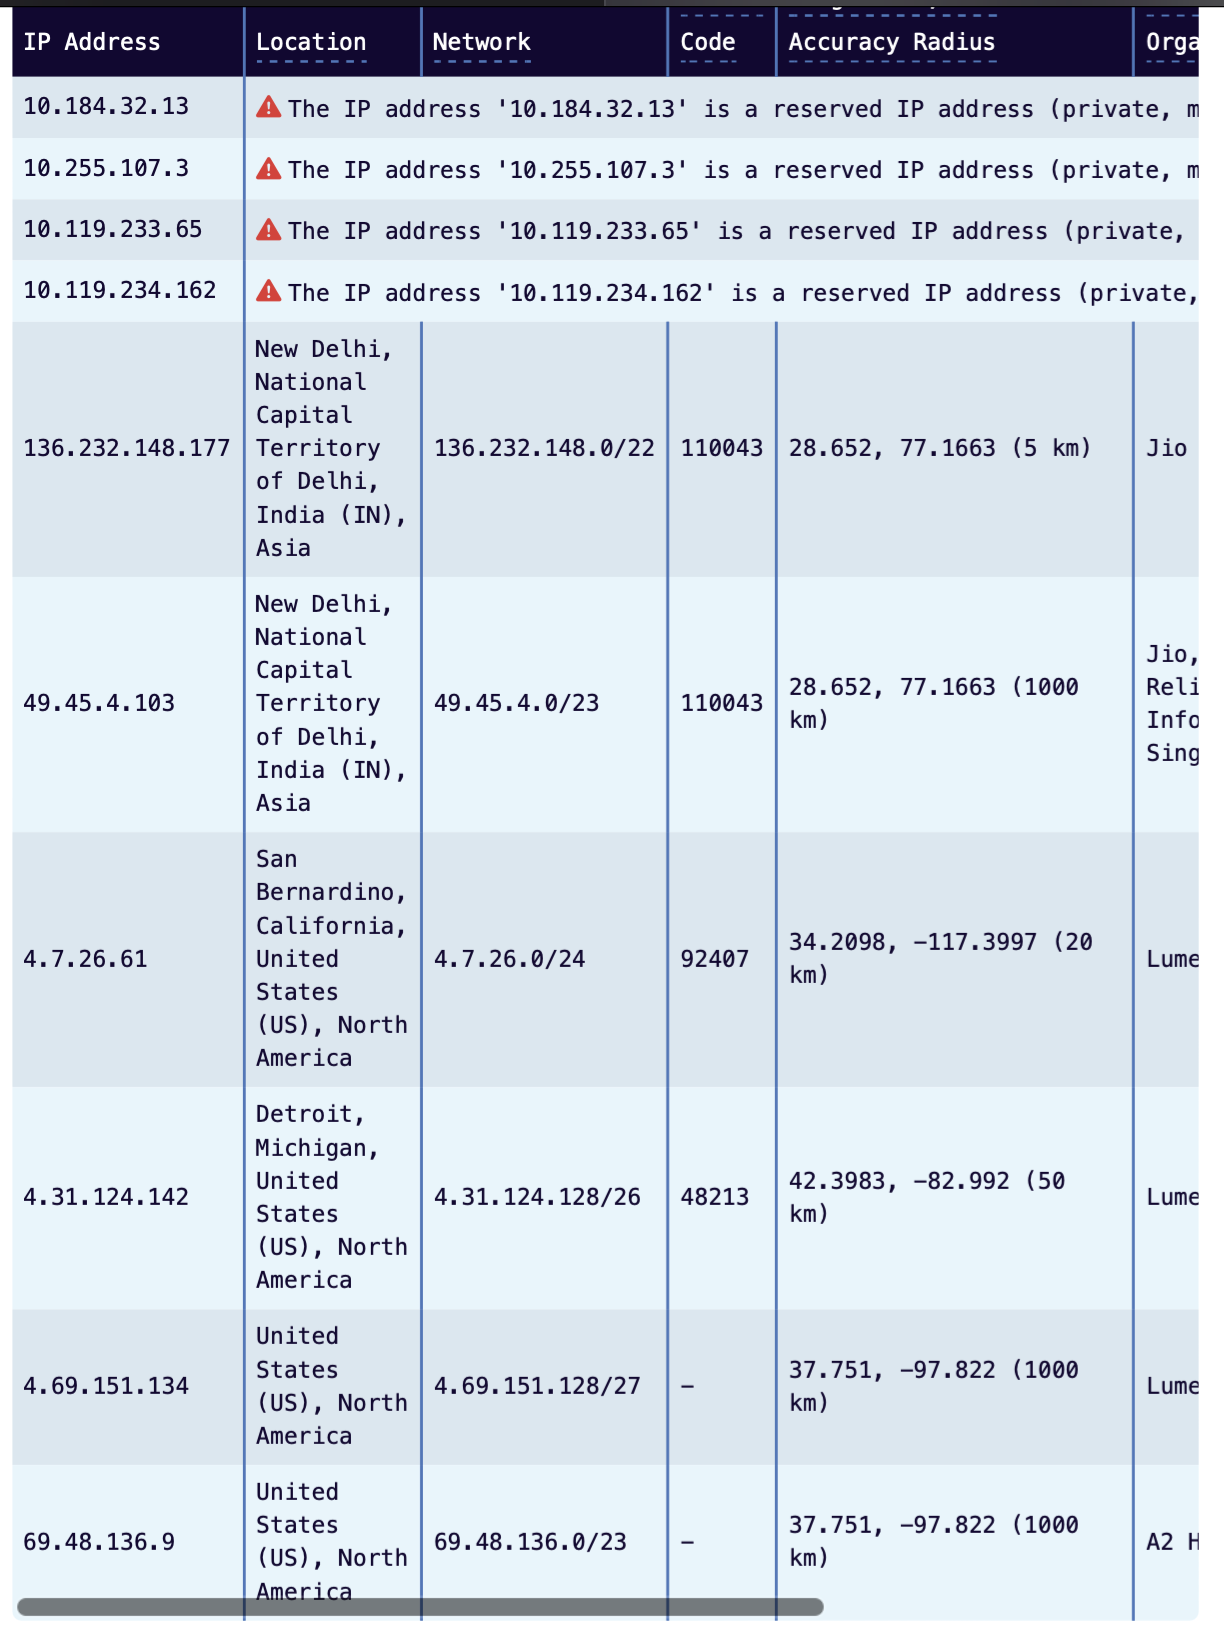
\includegraphics[width=0.9\textwidth]{geoloation_sigcomm_iitd.png}
    \caption*{Sigcomm with IITD Network}
    \end{figure}

    \begin{figure}[H]
    \centering
    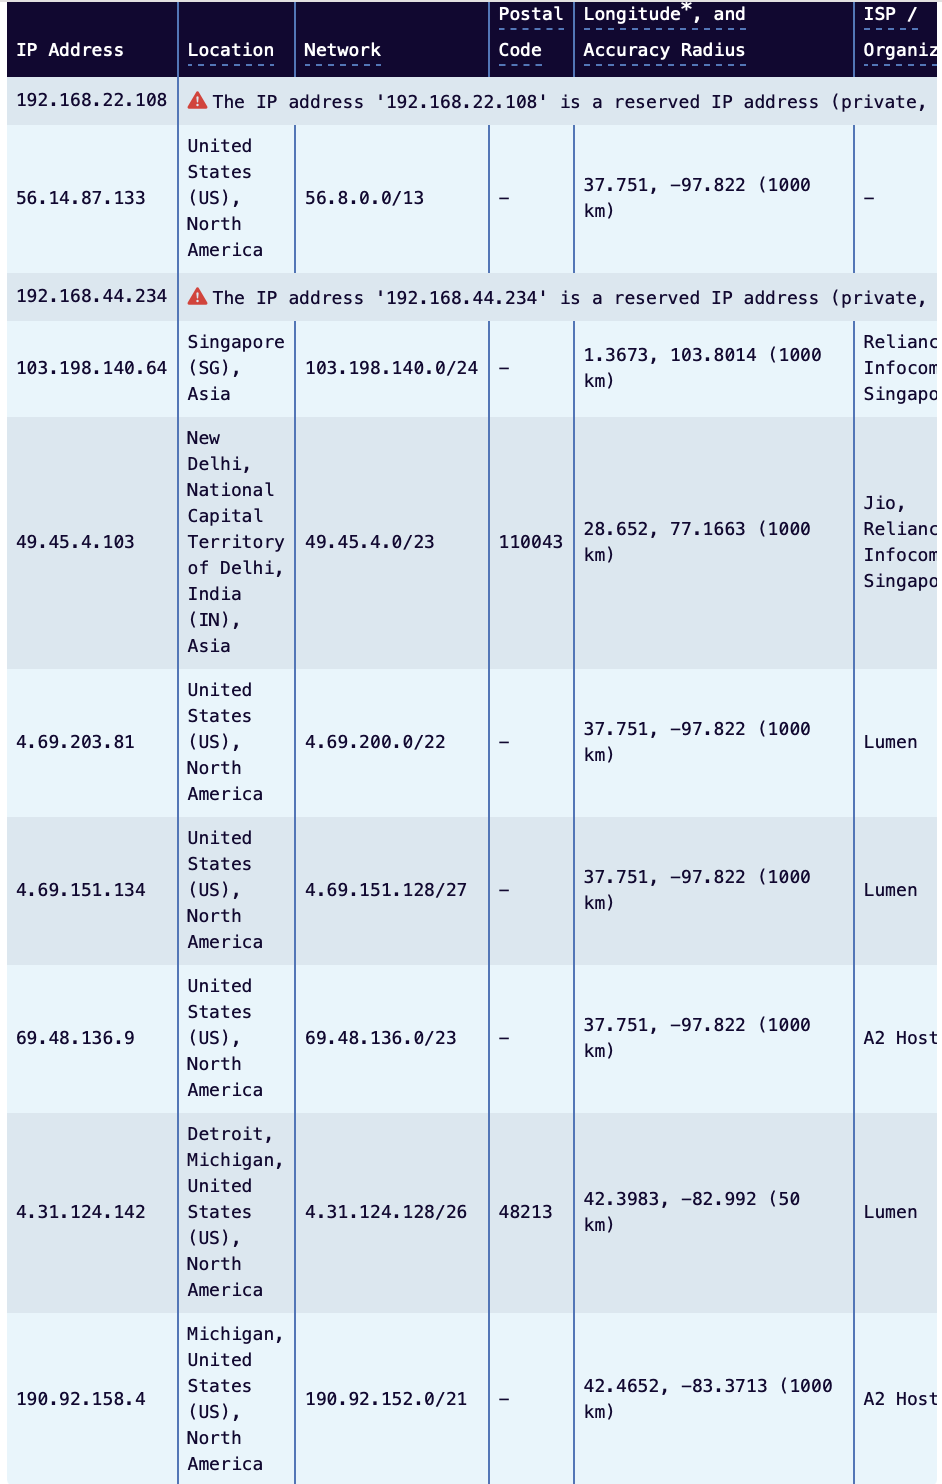
\includegraphics[width=0.9\textwidth]{geolocation_sigcomm_personal.png}
    \caption*{Sigcomm with personal network}
    \end{figure}
\end{itemize}

\newpage

\section{Network Data Collection and Header Analysis}
We used Wireshark to collect the network traffic for the 2-person MS Teams video call.

This is the link for PCAP file:-
\href{https://csciitd-my.sharepoint.com/:u:/g/personal/cs5221133_iitd_ac_in/EXyzrXDXeWVHmEXI7Gj0ubYBvL5JNiTyRngBvNulR8BsNw?e=OwpG6S}{Click here}

\subsection{Protocols identified}
The following wireshark screenshot shows the protocols identified during the call.

    \begin{figure}[H]
    \centering
    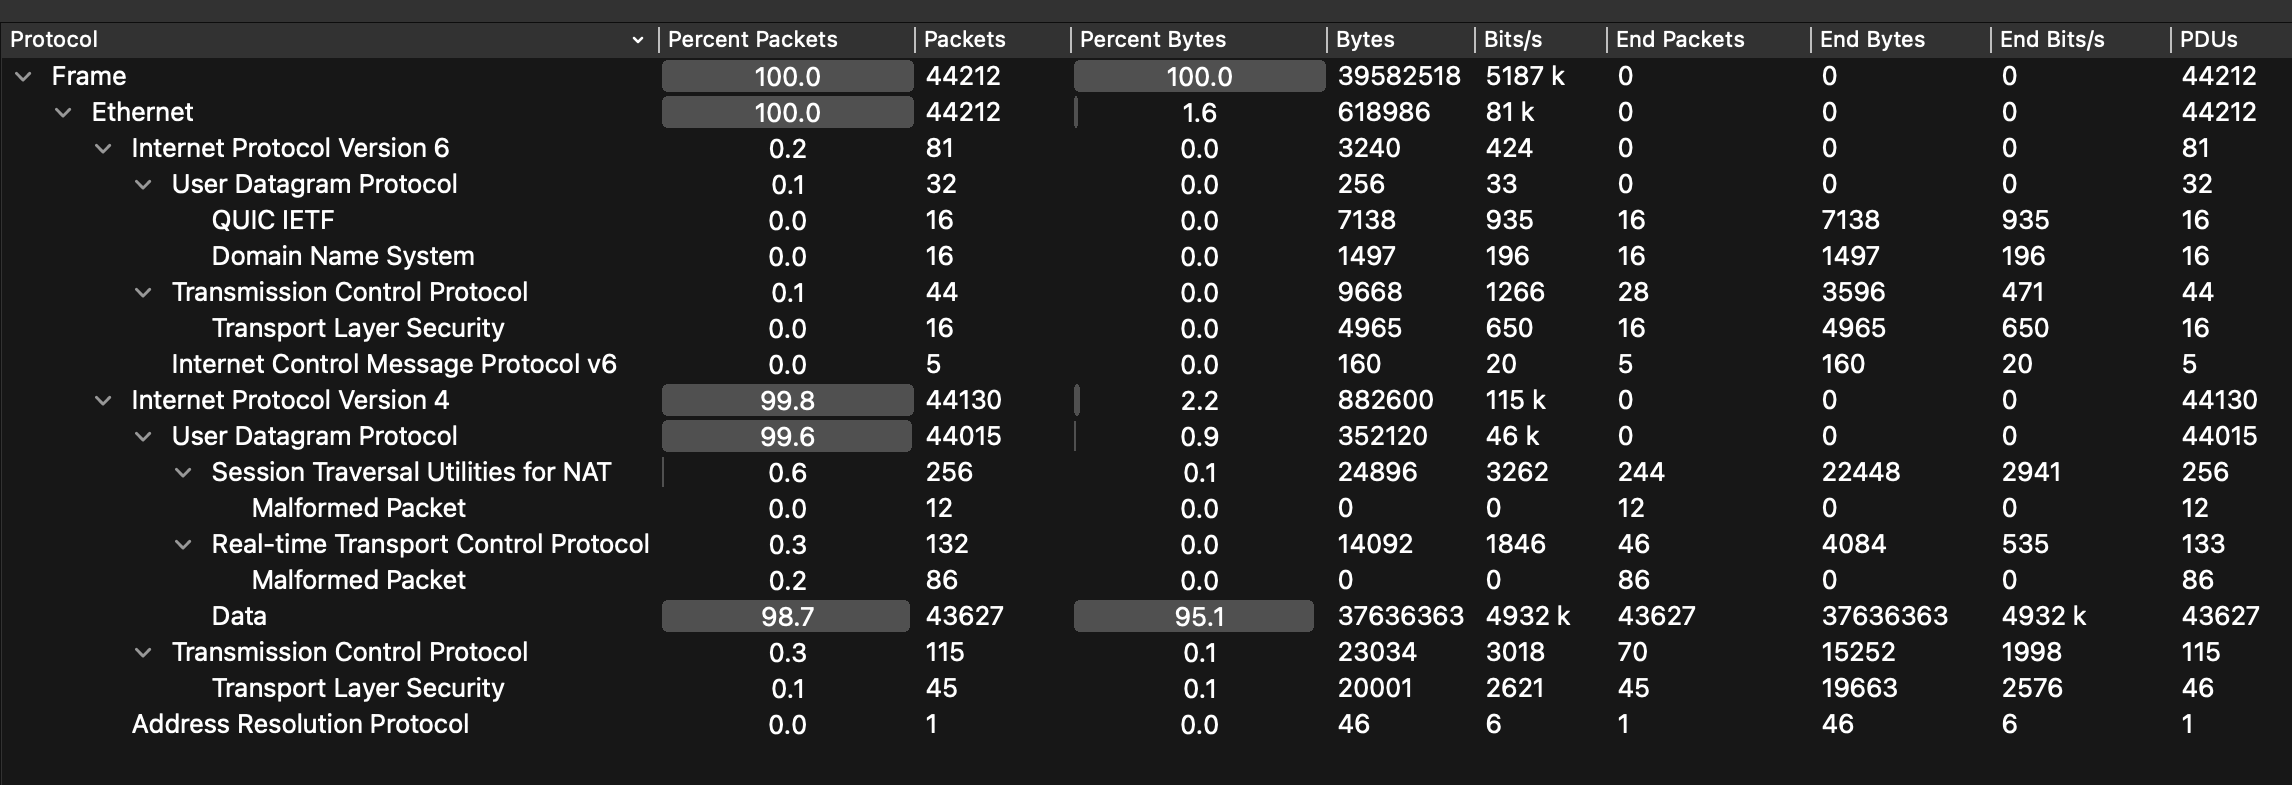
\includegraphics[width=\textwidth]{protocols.png}
    \caption*{Procols detected}
    \end{figure}

\begin{itemize}
    \item Link layer protocol :- Ethernet (used by IITD Wifi):- 100 \%
    \item Network layer protocols
        \begin{enumerate}
            \item IPv4:- used by MS teams
            \item IPv6:- background traffic
        \end{enumerate}
    \item Transport layer protocol:- User Datagram Protocol (UDP):- 100 \%
    \item Application layer protocols
        \begin{enumerate}
            \item Session traversal utilities for NAT (STUN):- 0.6 \%
            \item Real-time transport control protocol (RTCP):- 0.3 \%
        \end{enumerate}
    
\end{itemize}

\subsection{Direct connection between hosts}
Yes, we observed a direct connection between the two hosts. This is visible as the source and destination IP addresses match the IP addresses of my and my partner's computers. 

    \begin{figure}[H]
    \centering
    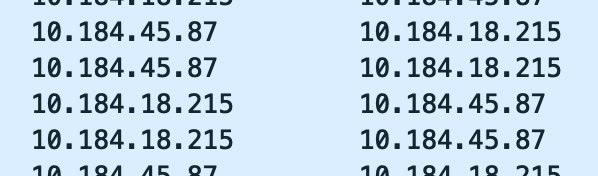
\includegraphics[width=0.9\textwidth]{direct_connection.png}
    \caption*{Source and destination IPs}
    \end{figure}

\begin{figure}[H]
    \centering
    \begin{subfigure}[b]{0.465\textwidth}
        \centering
        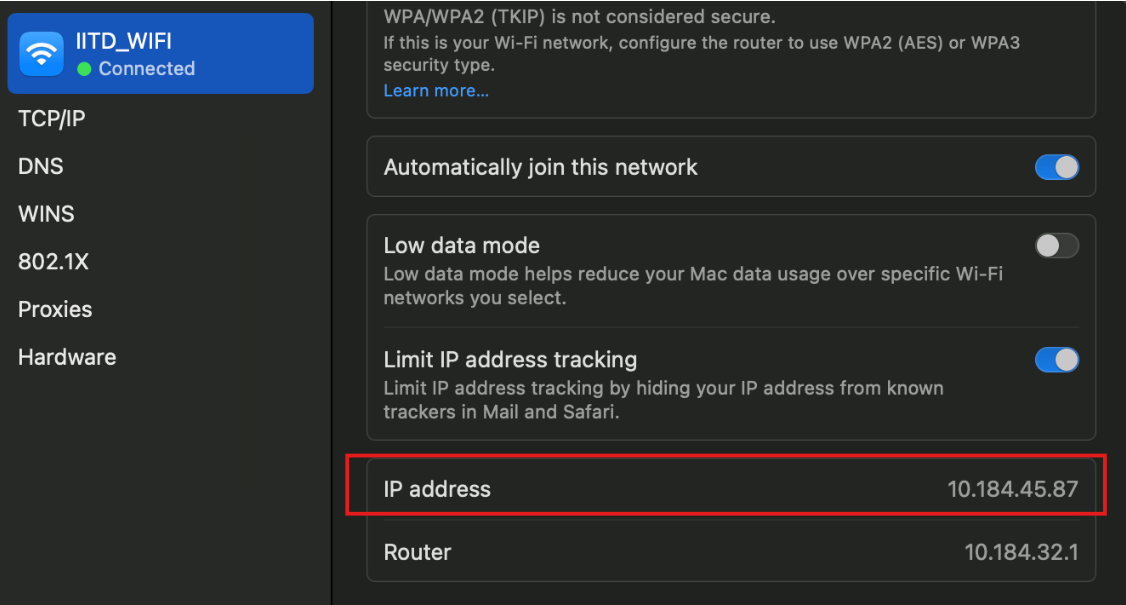
\includegraphics[width=\textwidth]{yash_ip.png}
        \caption*{\textbf{My IP address}}
    \end{subfigure}
    \hfill
    \begin{subfigure}[b]{0.50\textwidth}
        \centering
        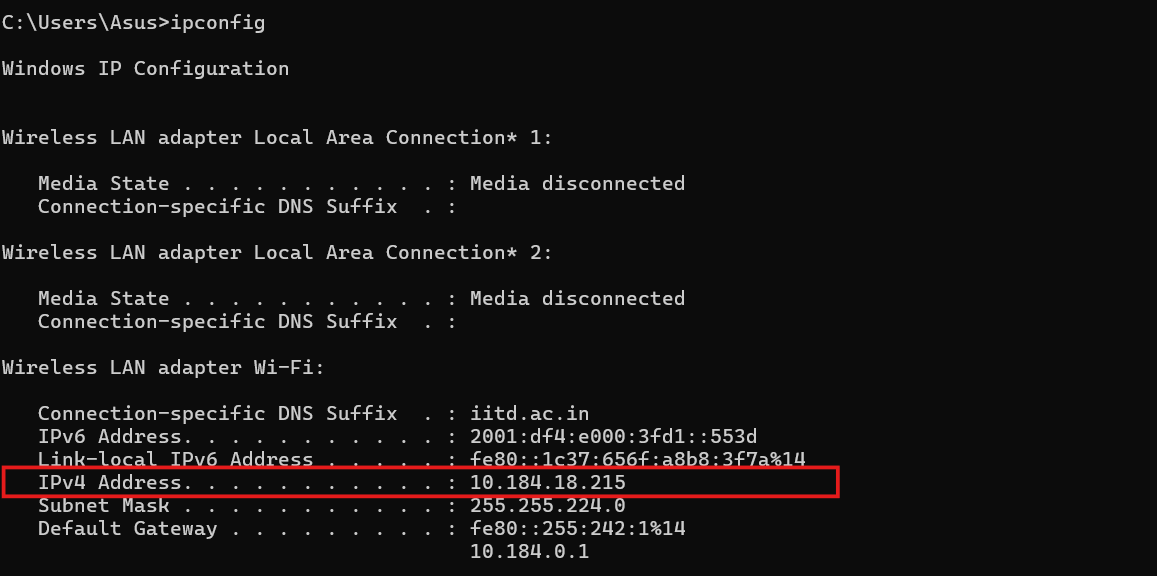
\includegraphics[width=\textwidth]{nikhil_ip.png}
        \caption*{\textbf{Partner's IP address}}
    \end{subfigure}
\end{figure}

\subsection{Filtering Audio and Video packets}
We filtered the audio and video packets using the following logic:-
\begin{itemize}
    \item When we kept only videos on both ends, the UDP packets of only size greater than 500 were captured by Wireshark.
    \item On the other hand, when only audio was kept on, only the packets of size less than 300 were captured.
    \item When both were kept on, all the types of UDP packets occurred.
    \item Also, for audio packets, when we were not speaking, audio packets were of size less than 100. While speaking, audio packets are larger than 100 but less than 400.
    \item When both audio and videos are kept off, no UDP packets are detected. This procedure confirms that MS teams only use UDP packets of the size described above for audio and video.
\end{itemize}

\textbf{Observations:-} 
\begin{itemize}
    \item Total audio and video packets captured:- 44003
    \item Total audio packets captured:- 6499
    \item Total video packets captured:- 37504
    \item \% audio packets:- 14.76 \%
    \item \% video packets:- 85.23 \%
\end{itemize}

\begin{figure}[H]
    \centering
    \begin{subfigure}[b]{0.48\textwidth}
        \centering
        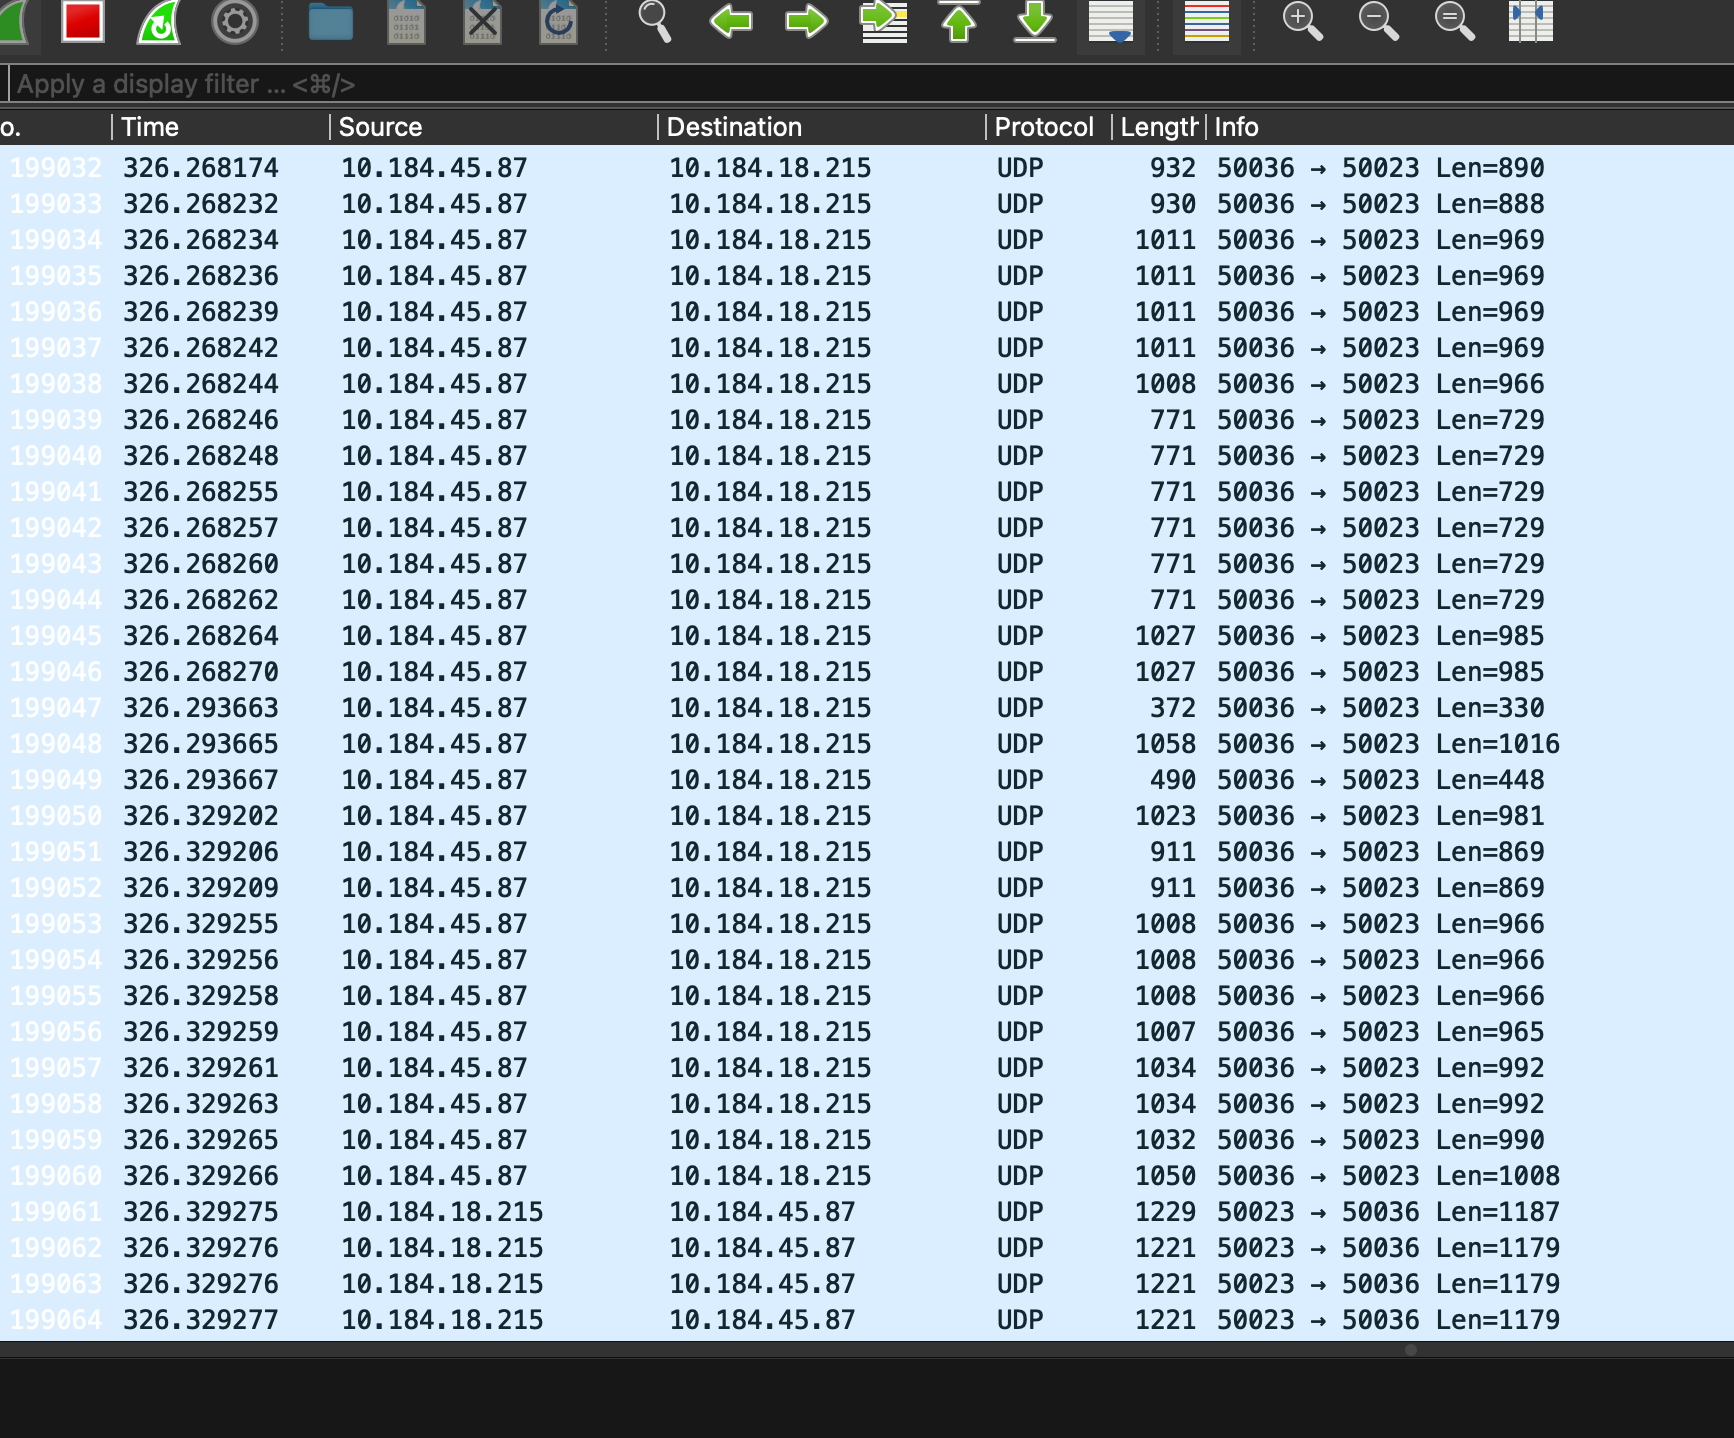
\includegraphics[width=\textwidth]{only_video.png}
        \caption*{\textbf{Only video on}}
    \end{subfigure}
    \hfill
    \begin{subfigure}[b]{0.465\textwidth}
        \centering
        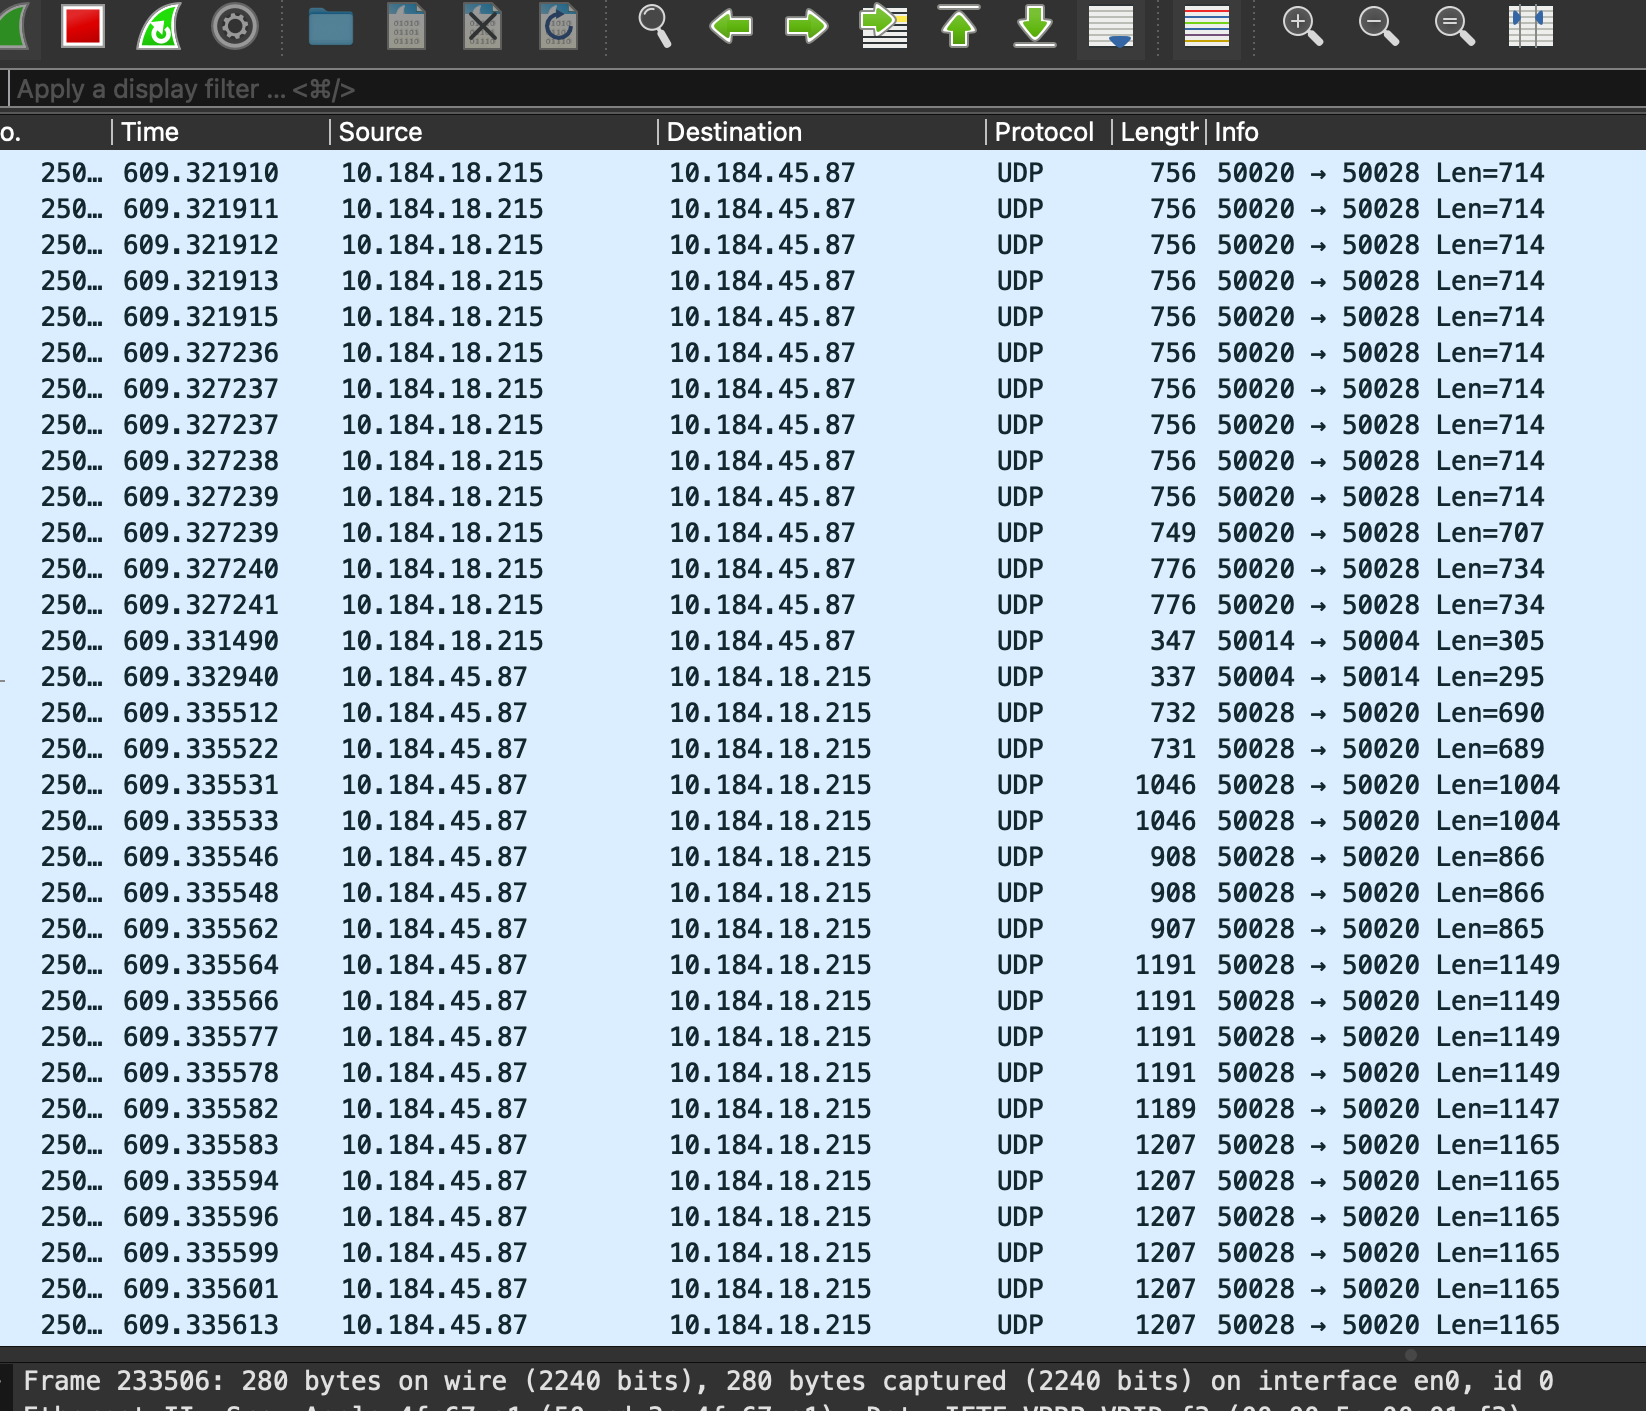
\includegraphics[width=\textwidth]{audio_and_video.png}
        \caption*{\textbf{Both audio and video on}}
    \end{subfigure}

\end{figure}

\begin{figure}[H]
    \centering
    \begin{subfigure}[b]{0.455\textwidth}
        \centering
        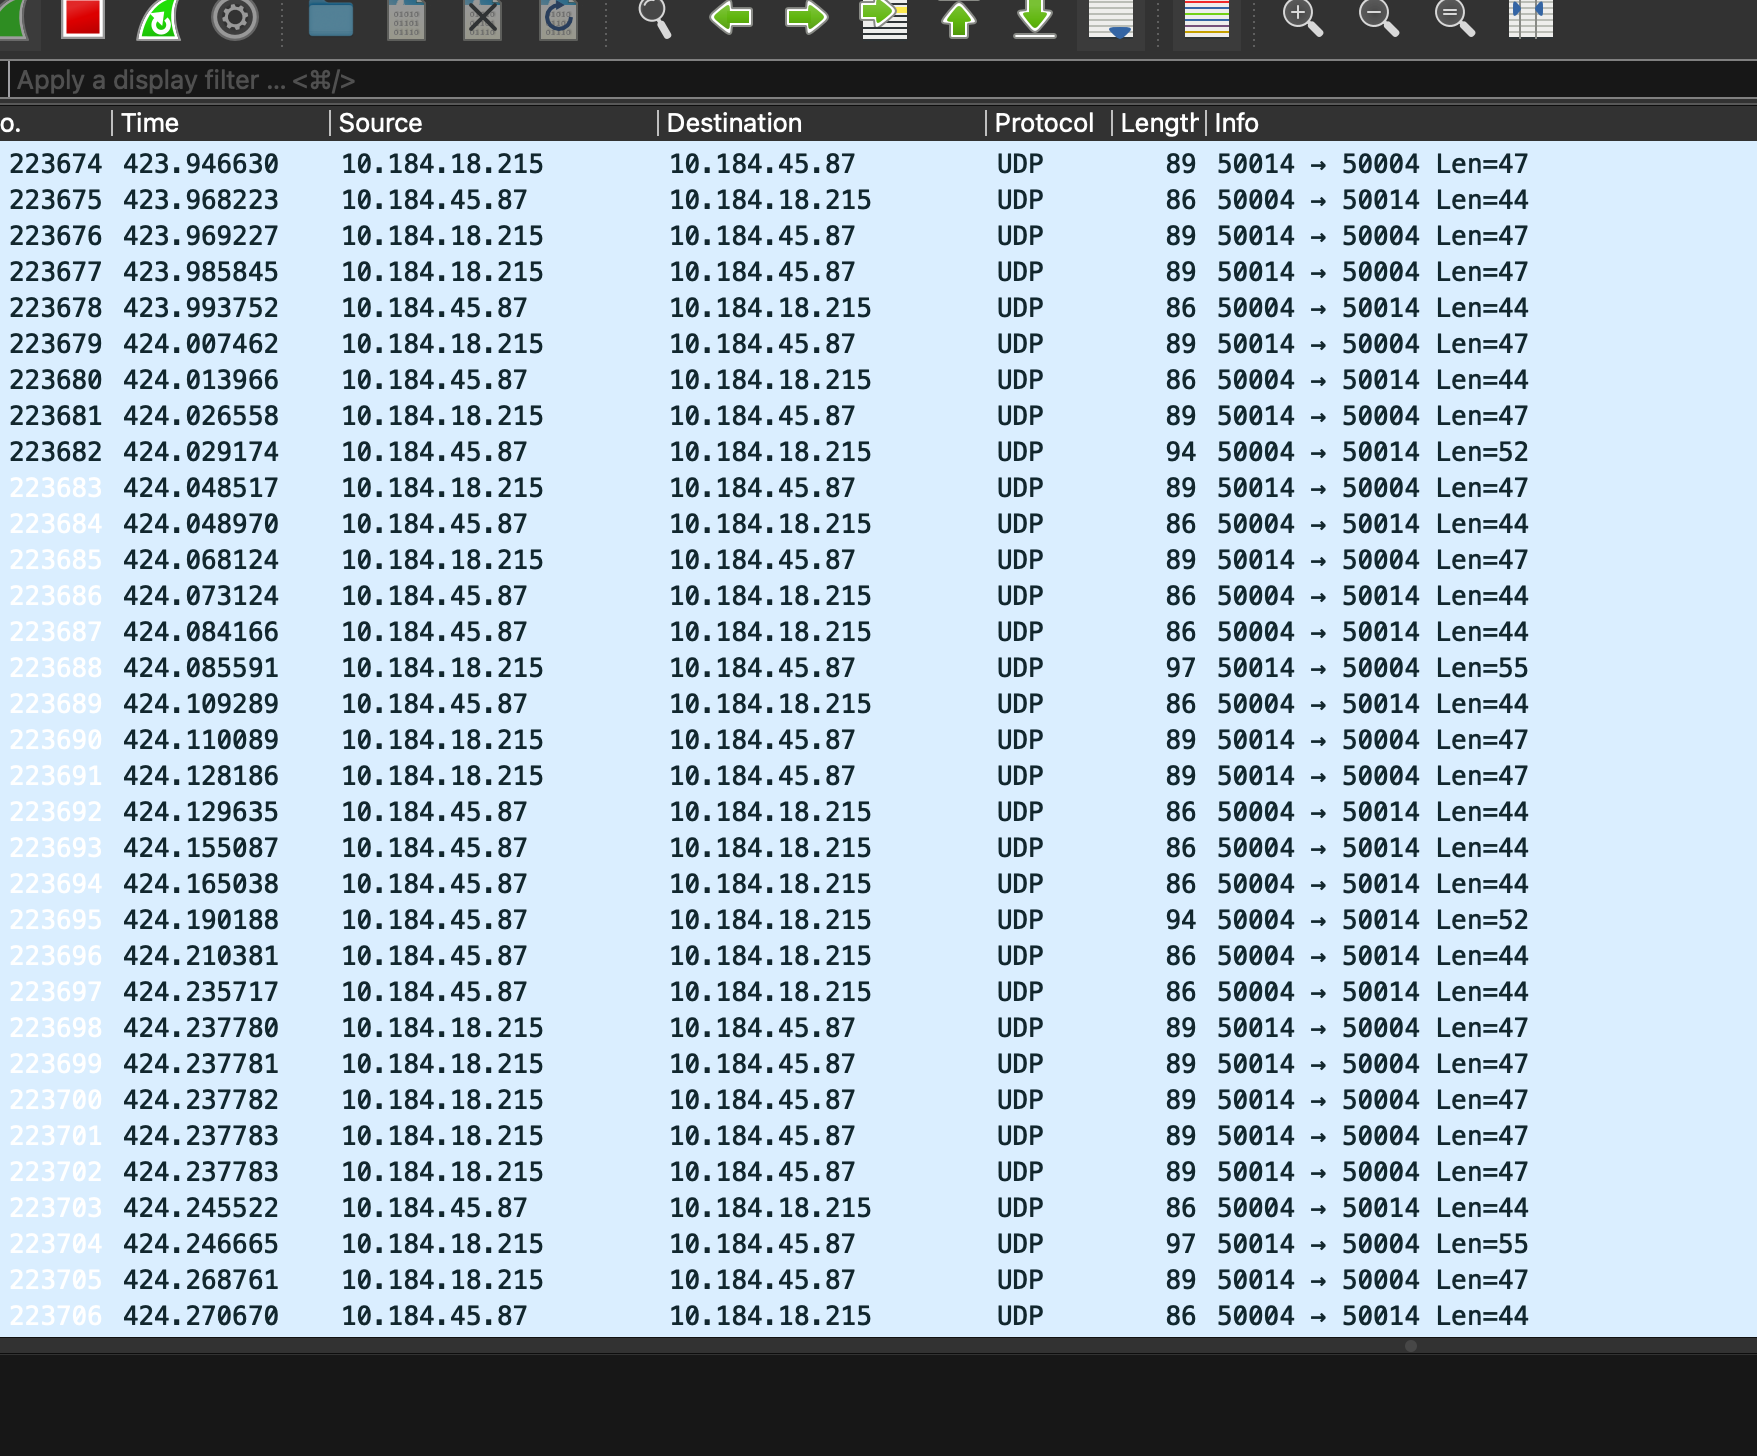
\includegraphics[width=\textwidth]{only_audio_no_speaking.png}
        \caption*{\textbf{Only audio on with speaking without speaking}}
    \end{subfigure}
    \hfill
    \begin{subfigure}[b]{0.48\textwidth}
        \centering
        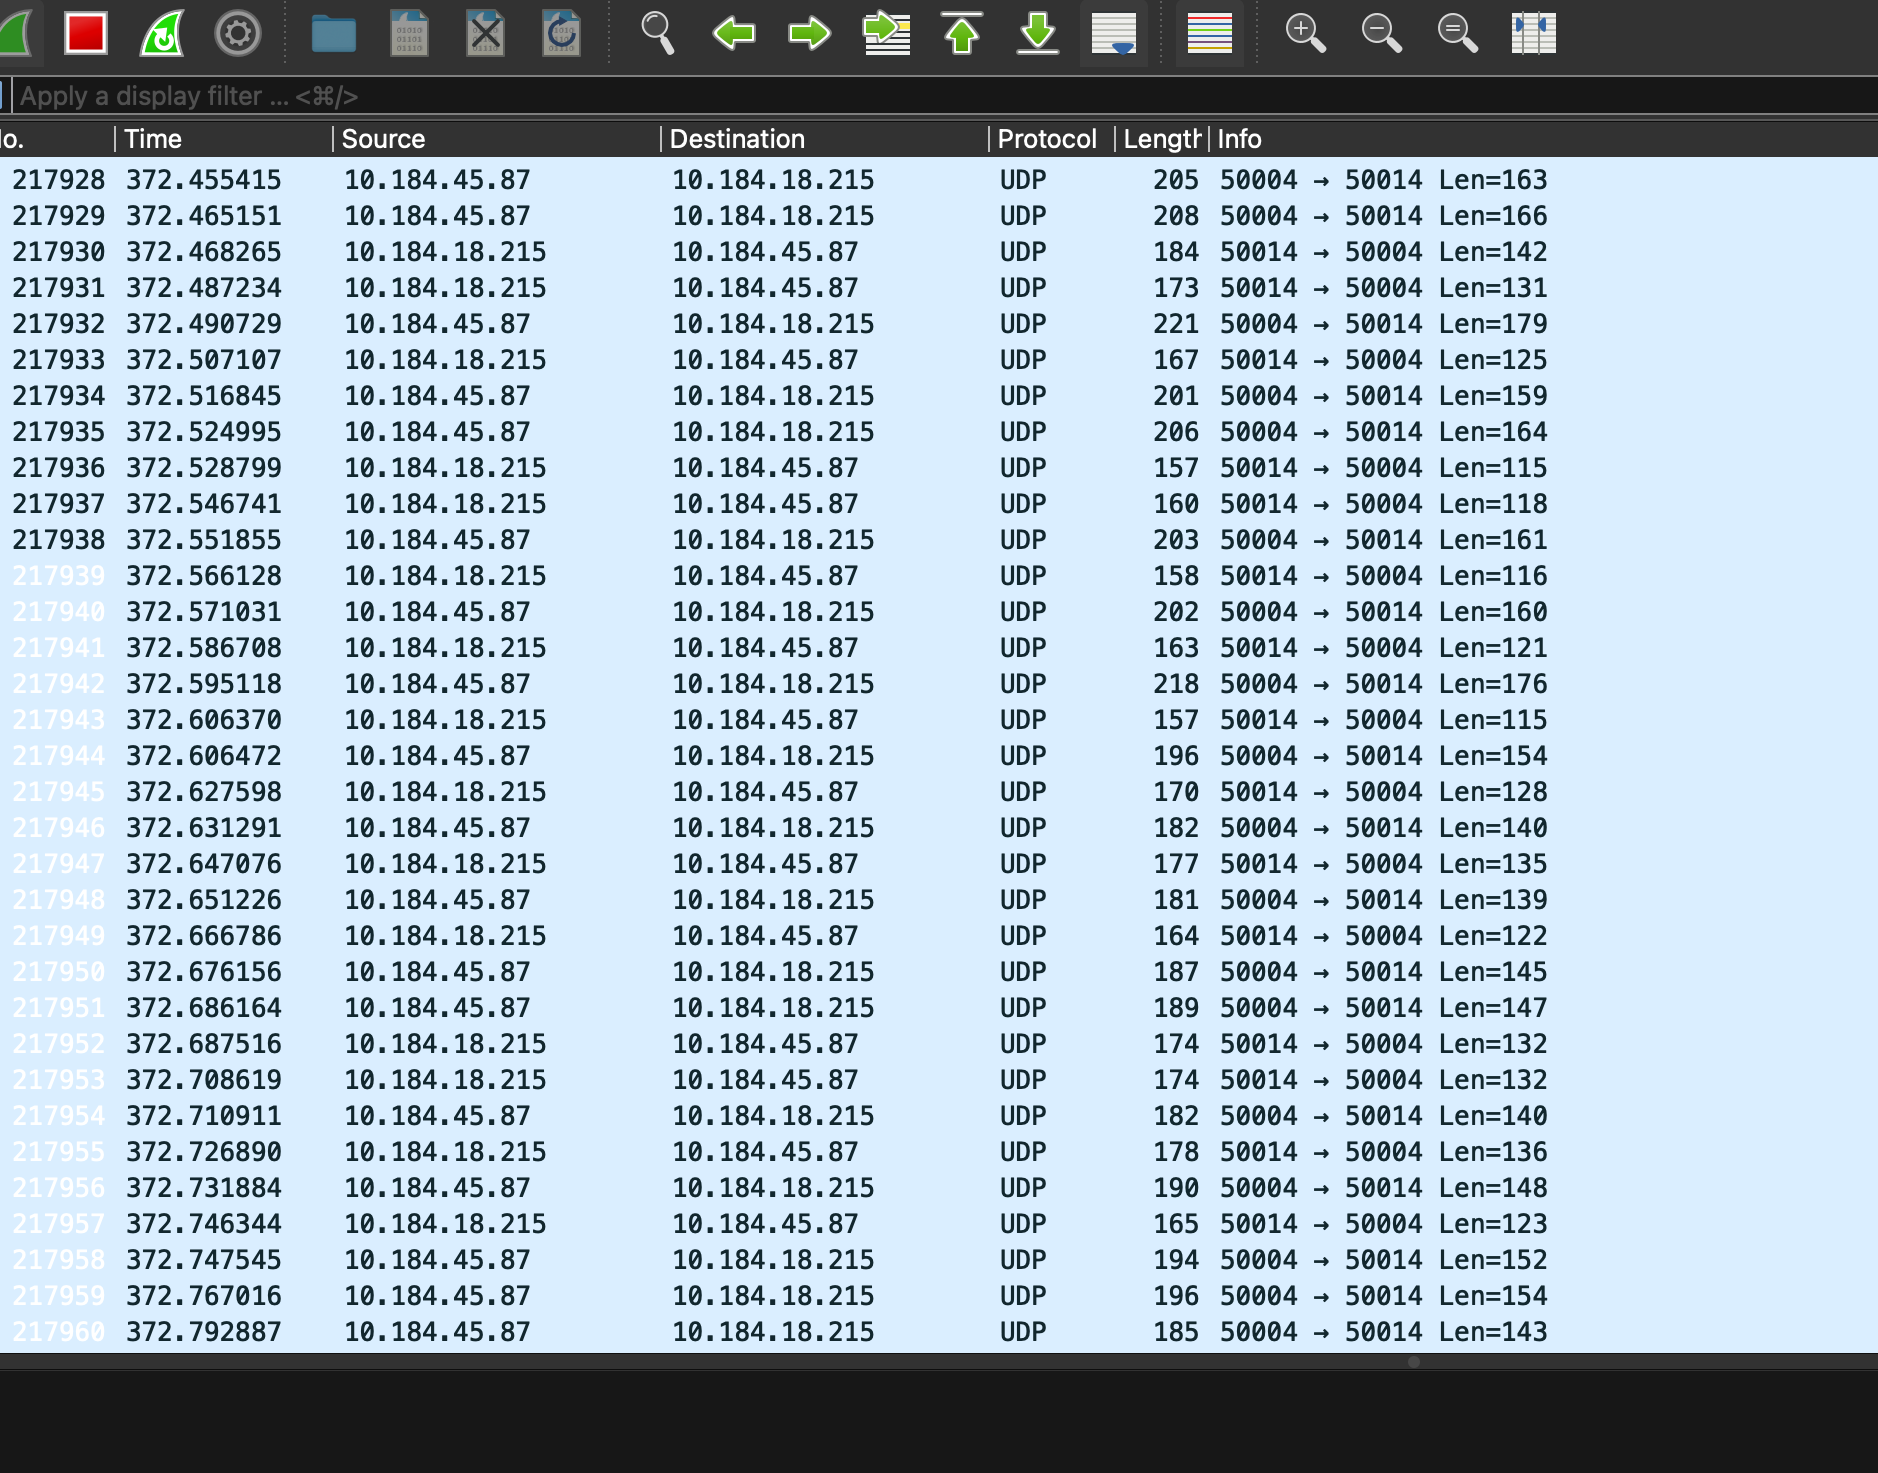
\includegraphics[width=\textwidth]{only_audio_speaking.png}
        \caption*{\textbf{Only audio on with speaking}}
    \end{subfigure}
\end{figure}

\textbf{Bandwitdh Utilisation:-}

Green:- Video packets

brown:- Audio packets

    \begin{figure}[H]
    \centering
    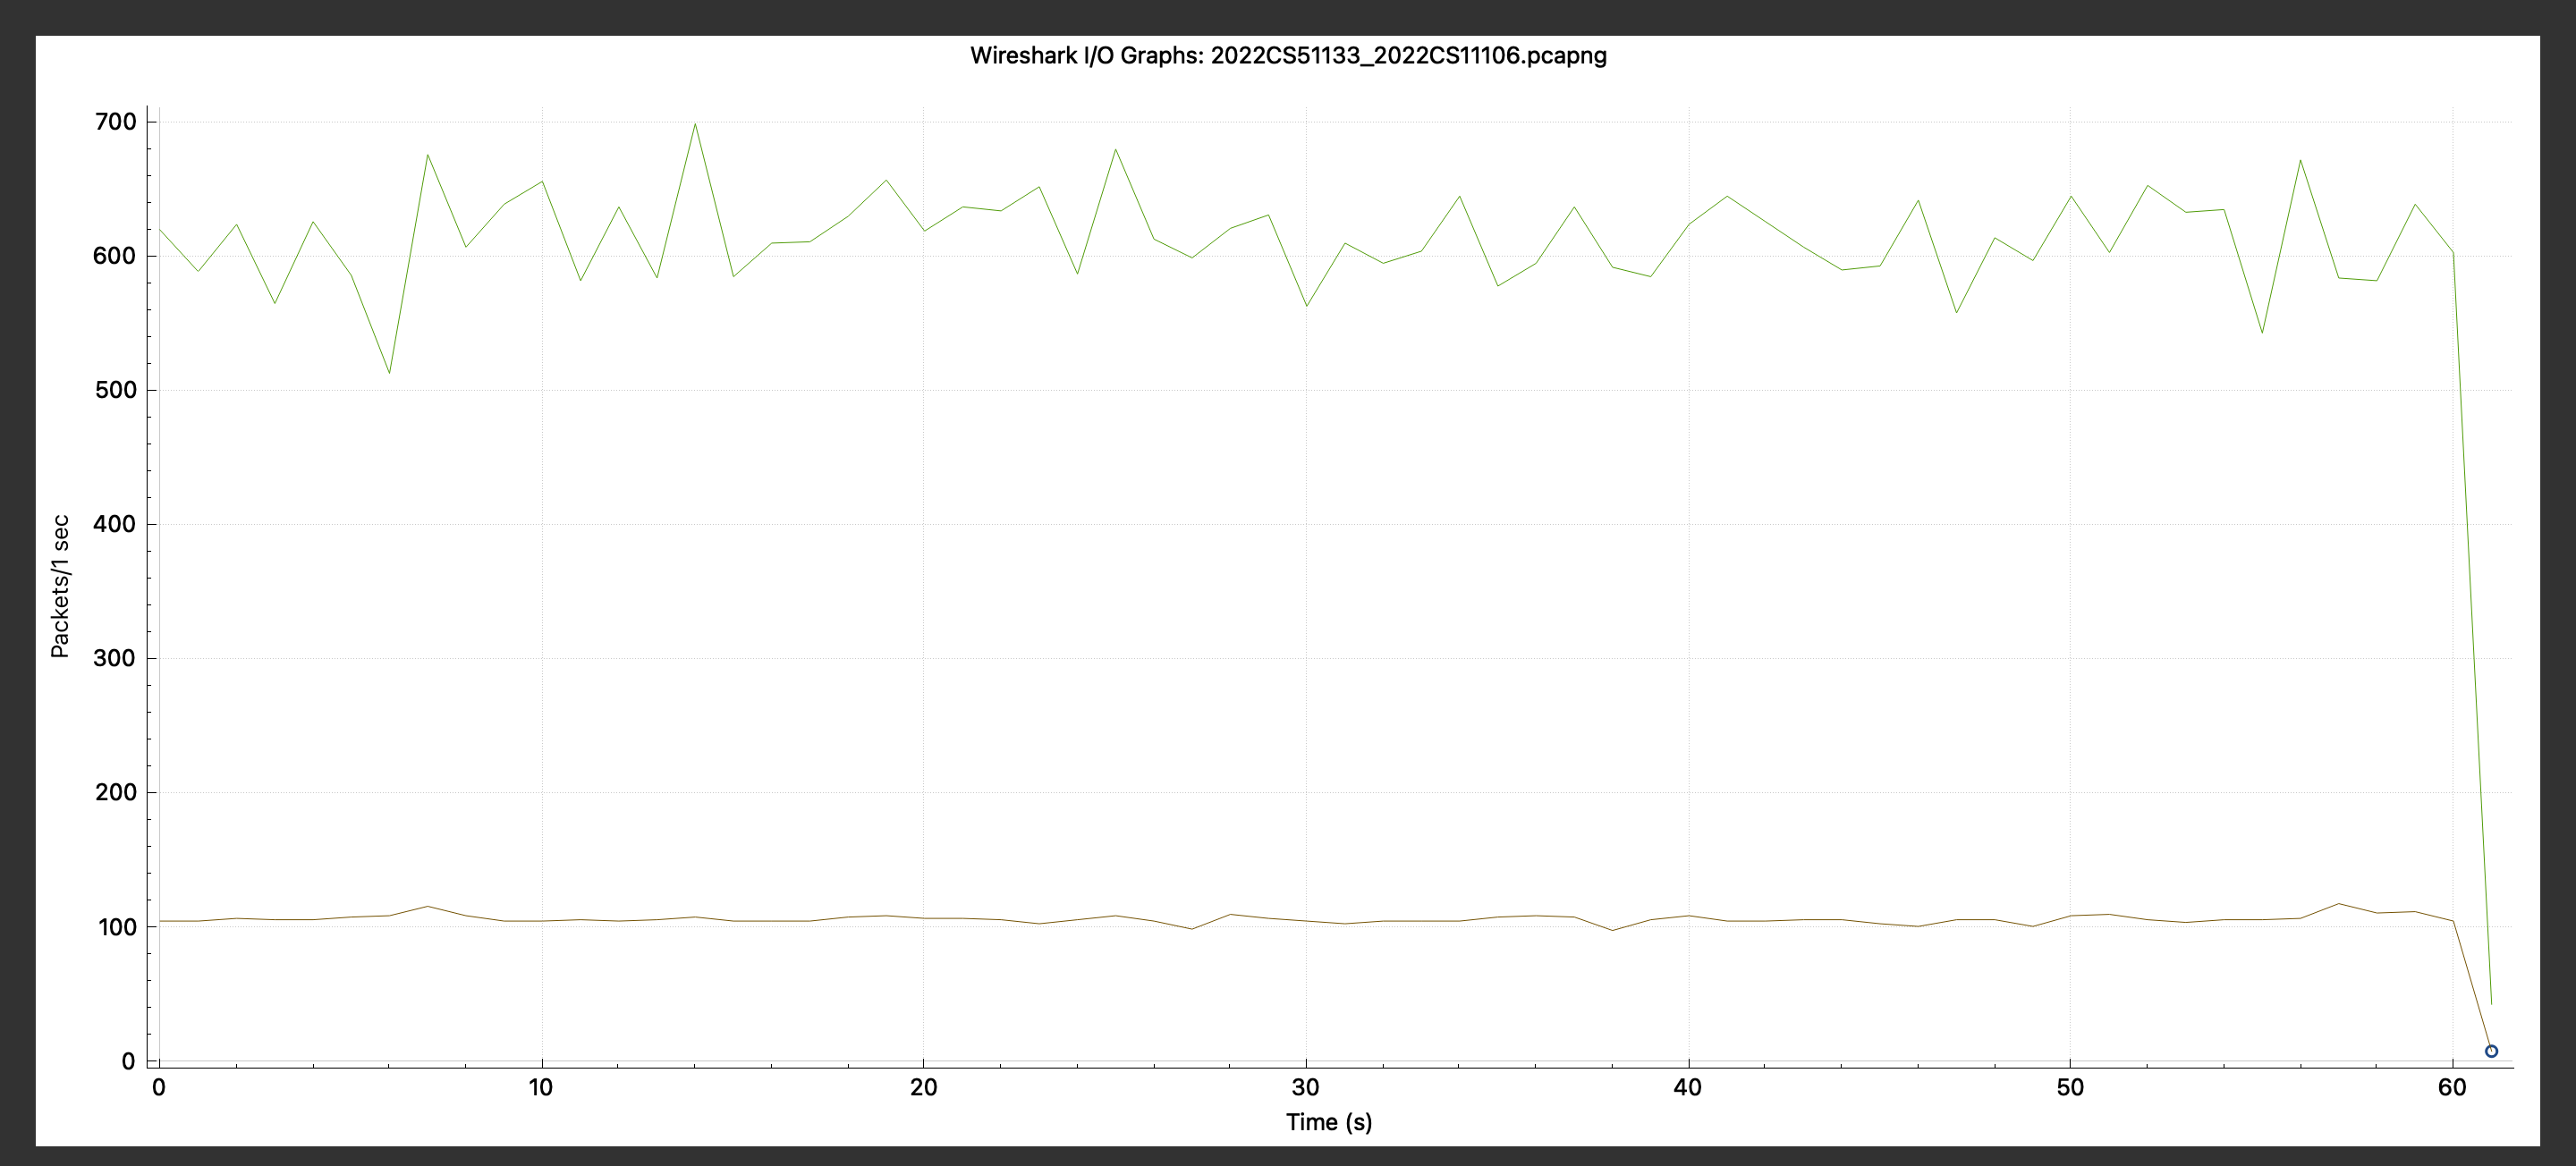
\includegraphics[width=\textwidth]{bandwitdh_graph.png}
    \caption*{Bandwitdh Utilisation by Audio and Video}
    \end{figure}
    
\newpage

\section{Traffic Analysis and Network Performance}
I used \textbf{dpkt} python library to read the given .pcapng file of the NDT7 speed test. On analyzing the given speed test file and a speed file I created using Wireshark, it can be seen that the NDT7 test handshakes 4 times during the complete speed test. In these 4 handshakes, the first is downloaded, and the second is uploaded to one IP address. Download and upload are done using a different IP address for the next two handshakes. NDT7 tests our network on two IP addresses for upload and download. The speed test file given to us truncates after the second download procedure, as seen in the graph below.
\subsection{Percentage Traffic}
The NDT7 test uses TCP transport protocol and has port 443 on its server. So, the first filter is done based on protocol and port. Also, the packets which do not have any source/destination IP address are removed. The distinction between upload and download packets is based on the source and destination ports. Upload packets have destination port 443, while download packets have source port 443.


\textbf{Percentage packets traffic for speed test:- 86.82 \%}

\textbf{Percentage bytes traffic for speed test:- 88.45 \%}

\subsection{Throughput}
Upload and download packets are separated based on the port to calculate throughput. Then, for each second from the start of the file, the packets are accumulated for each second for both upload and download and then the graph is plotted. The following is the throughput graph for the given speed test file.

    \begin{figure}[H]
    \centering
    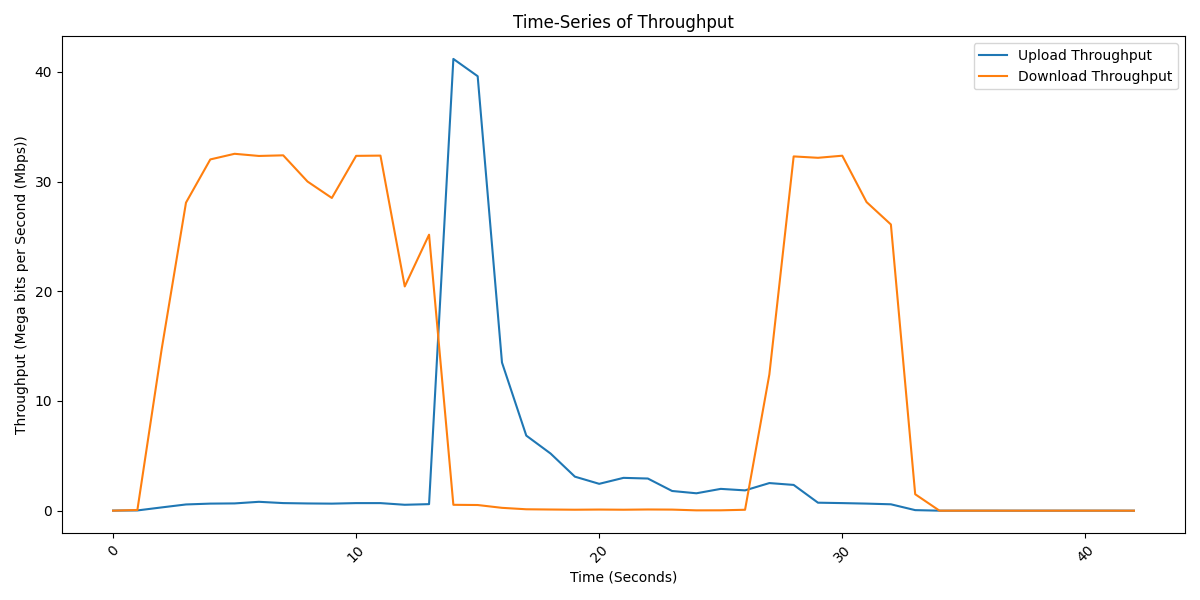
\includegraphics[width=\textwidth]{avg_throughput.png}
    \caption*{Throughput graph for upload and download}
    \end{figure}

\subsection{Upload and Download speed}
For calculating the speed of upload/download, the maximum throughput per second is calculated, and then only that particular time frame is considered for which the throughput is greater than 25 \%. This is because, at other times, it can be fairly assumed that the speed test was on the other phase. 

\textbf{Download speed in Megabits per second:- 28.023 Mbps}

\textbf{Upload speed in Megabits per second:- 31.432 Mbps}
\end{document}